\documentclass{beamer}
\usepackage{tikz,tabularx,booktabs}
\graphicspath{{./figures/}}
\usetikzlibrary{decorations,arrows,shapes,positioning}
\tikzset{variable/.default=}
\usepackage{biblatex}
\renewcommand{\footnotesize}{\scriptsize}
\newrobustcmd*{\footlessfullcite}{\AtNextCite{\renewbibmacro{title}{}\renewbibmacro{note+pages}{}\renewbibmacro{in:}{}}\footfullcite}

\definecolor{dkgreen}{rgb}{0,0.6,0}
\definecolor{gray}{rgb}{0.5,0.5,0.5}
\definecolor{purple}{rgb}{0.73,0.33,0.83}
\definecolor{aoi}{RGB}{105,210,231}
\definecolor{goldfish}{RGB}{243,134,48}
\definecolor{beachstorm}{RGB}{224,228,204}
\definecolor{pondwater}{RGB}{167,219,216}
% Warming Up
\definecolor{purpderp}{RGB}{53,12,31}
\definecolor{dred}{RGB}{141,27,22}
\definecolor{borange}{RGB}{192,54,0}
\definecolor{bage}{RGB}{255,255,183}
\definecolor{peas}{RGB}{129,153,6}
% My Own
\definecolor{lblue}{RGB}{153,229,255}
\definecolor{llblue}{RGB}{192,246,255}

\useinnertheme{rectangles}
% \useoutertheme{default}
\setbeamertemplate{footline}[frame number]
\setbeamertemplate{blocks}[rounded][shadow=true]
\setbeamertemplate{background canvas}[vertical shading][bottom=lblue!30!white,top=llblue!20!white]
\setbeamercolor{alerted text}{fg=goldfish}
% \setbeamercolor{background canvas}{bg=bage!70!white}
\setbeamercolor{block body alerted}{bg=normal text.bg!90!black}
\setbeamercolor{block body}{bg=normal text.bg!90!black}
\setbeamercolor{block body example}{bg=normal text.bg!90!black}
\setbeamercolor{block title alerted}{use={normal text,alerted text},fg=alerted text.fg!75!normal text.fg,bg=normal text.bg!75!black}
\setbeamercolor{block title}{bg=peas}
\setbeamercolor{block title example}{use={normal text,example text},fg=example text.fg!75!normal text.fg,bg=normal text.bg!75!black}
\setbeamercolor{fine separation line}{}
\setbeamercolor{frametitle}{fg=white, bg=borange}
\setbeamercolor{item projected}{fg=black}
\setbeamercolor{itemize item}{fg=peas}
\setbeamercolor{normal text}{fg=black}
\setbeamercolor{palette sidebar primary}{use=normal text,fg=normal text.fg}
\setbeamercolor{palette sidebar quaternary}{use=structure,fg=structure.fg}
\setbeamercolor{palette sidebar secondary}{use=structure,fg=structure.fg}
\setbeamercolor{palette sidebar tertiary}{use=normal text,fg=normal text.fg}
\setbeamercolor{section in sidebar}{fg=brown}
\setbeamercolor{section in sidebar shaded}{fg= grey}
\setbeamercolor{separation line}{}
\setbeamercolor{sidebar}{bg=red}
\setbeamercolor{sidebar}{parent=palette primary}
\setbeamercolor{structure}{bg=black, fg=black}
\setbeamercolor{subsection in sidebar}{fg=brown}
\setbeamercolor{subsection in sidebar shaded}{fg= grey}
\setbeamercolor{title}{fg=dred,bg=}
\setbeamercolor{titlelike}{fg=black}
\setbeamercolor{footnote}{fg=black}
% \beamertemplatenavigationsymbolsempty

\bibliography{thesis}

\title{Brain tissue temperature dynamics during functional activity and possibilities for optical measurement techniques}
\author{Greggory Rothmeier}
\institute{
  Department of Physics and Astronomy\\
  Georgia State University\\
  Atlanta, GA 30303\\
}
\date{April 3, 2012}

\newcommand{\degree}{\ensuremath{^\circ}}
\begin{document}

%  * What is BOLD?
%  * Temperature
%     * Experimental Measurements
%     * Modeling
%        * Previous Models
%        * Our Model
%  * Optical Techniques
%     * fNIRS
%     * Thermal Imaging
%  * Conclusion/Future Work
  
  
{
\setbeamercolor{background canvas}{bg=dred}
\setbeamercolor{text}{fg=white}
\begin{frame}[plain]
\titlepage
\end{frame} 
}

\frame{
\frametitle{Outline}
  \begin{itemize}
           \item fMRI and BOLD
    \pause \item Previous temperature models
    \pause \item Our approach
    \pause \item Optical techniques
  \end{itemize}
}

%%%%%%%%%%%%%%%%%%%%%%%%%%%%%%%%%%%%%%%%%%%%%%%%%%%%%%%%%%%%%%%
%%%%%  fMRI and BOLD
%%%%%%%%%%%%%%%%%%%%%%%%%%%%%%%%%%%%%%%%%%%%%%%%%%%%%%%%%%%%%%%

\frame{
\frametitle{fMRI and BOLD}
  Hemoglobin responds to the fMRI's magnetic field differently depending on the oxidative state:
  \begin{itemize}
    \item Deoxygenated: paramagnetic
    \item Oxygenated: diamagnetic
  \end{itemize}
  Deoxyhemoglobin alters the local magnetic susceptibility, thereby producing a slight change in the local MR signal.
}

\frame{
\frametitle{fMRI and BOLD: Local oxygen extraction fraction (E)}

\begin{columns}
  \column{0.7\linewidth}
  An increase in neuronal activity induces a much larger increase in cerebral blood flow (CBF) than the cerebral metabolic rate of oxygen (CMRO$_2$).
  
  \bigskip
  
  As a result, the local oxygen extraction fraction (E) decreases with activation~\footlessfullcite{fox1986}.
  
  \bigskip
  
  With less deoxy-hemoglobin present, the local MR signal increases and gives rise to a blood oxygenation level dependent (BOLD) signal change.
  
  \column{0.3\linewidth}
  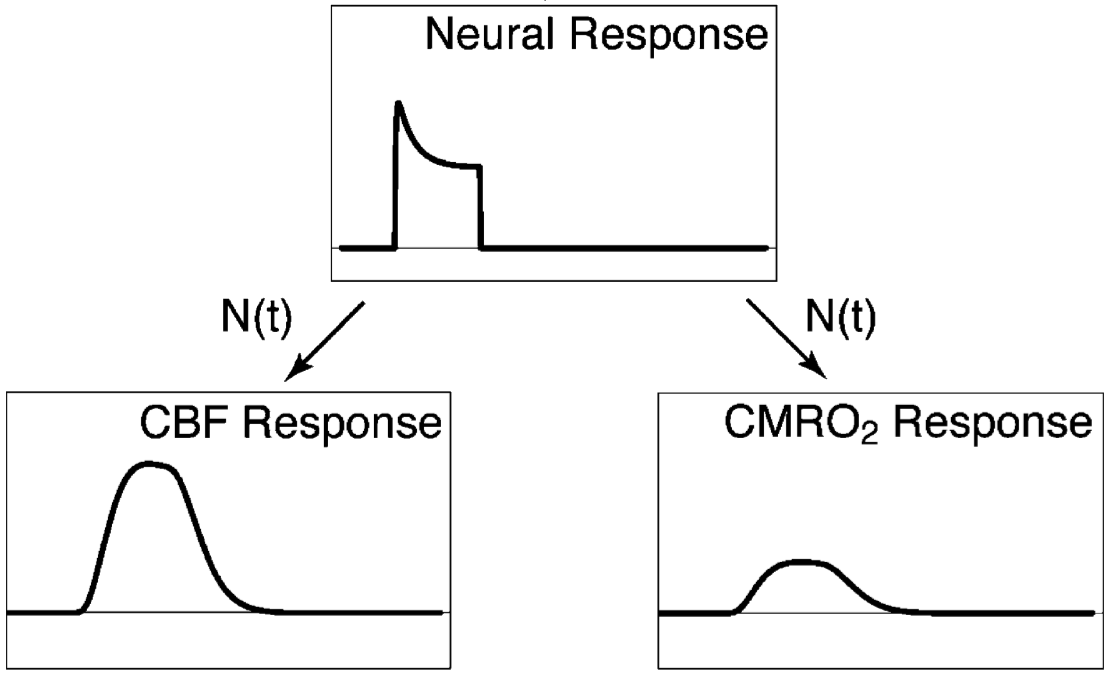
\includegraphics[width=\linewidth]{neuronal-cbf-cmro2-rastor}
\end{columns}

}

\frame{
\frametitle{Generation of the BOLD Response}
  \centering
  \resizebox{\textwidth}{!}{%
    \tikzstyle{block} = [draw=none, fill=beachstorm]
\tikzstyle{line} = [draw, very thick, color=black!50, -stealth']
\tikzstyle{sotero} = [draw, very thick, dashed, color=goldfish, -stealth']
\tikzstyle{collins} = [draw, very thick, dashed, color=aoi, -stealth']
\tikzstyle{citation} = [anchor=west, draw=none, align=left, minimum height=0.5cm, anchor=north, text width=4cm]

\begin{tikzpicture}[node distance=0.7cm, rectangle, text width=4.5cm, text badly centered, rounded corners, minimum height=1cm, anchor=north]
  \node[block](stimulus){Stimulus/Task};
  
  \node[block, below=of stimulus, xshift=-5cm](excitatory){Excitatory Neuronal Activity};
  \node[block, below=of stimulus, xshift= 7cm](inhibitory){Inhibitory Neuronal Activity};
  
  \node[block, below=of excitatory](cbf){Increase in Cerebral Blood Flow (CBF)};
  \node[block, below=of inhibitory, xshift=-3cm](o2){Change in Oxygen Consumption (CMRO$_2$)};
  
  \node[block, below=of cbf, xshift=4.5cm, yshift=-0.5cm](bold){fMRI BOLD Response};
  \node[block, below=of bold](temp){Temperature Change};
  
  \node[citation] at (-2.5, -5) {Sotero 2011};
  \node[citation] at (6.5, -6.5) {Collins 2004};
  
  \path[line](stimulus.west) -| (excitatory.north);
  \path[line](stimulus.east) -| (inhibitory.north);
  \path[line](excitatory.south) -- (cbf.north);
  \path[line](excitatory.east) -| (o2.north);
  \path[line](inhibitory.west) -| (o2.north);
  
  \path[line](cbf.south) |- ([yshift=-5pt] bold.west);
  \path[line](cbf.south) |- ([yshift= 5pt] temp.west);
  \path[line](o2.south)  |- ([yshift=-5pt] bold.east);
  \path[line](o2.south)  |- ([yshift= 5pt] temp.east);
  
  \path[sotero]([yshift= 5pt] bold) -| ([xshift= 20pt] cbf);
  \path[sotero]([yshift= 5pt] bold) -| ([xshift=-20pt] o2);
  \path[collins]([xshift=-45pt] cbf) |- ([yshift=-5pt] temp);
  \path[collins]([xshift=45pt] o2)  |- ([yshift= -5pt] temp);
\end{tikzpicture}
  }
}

\frame{
\frametitle{The Balloon Model}
  \centering
  \resizebox{\textwidth}{!}{%
    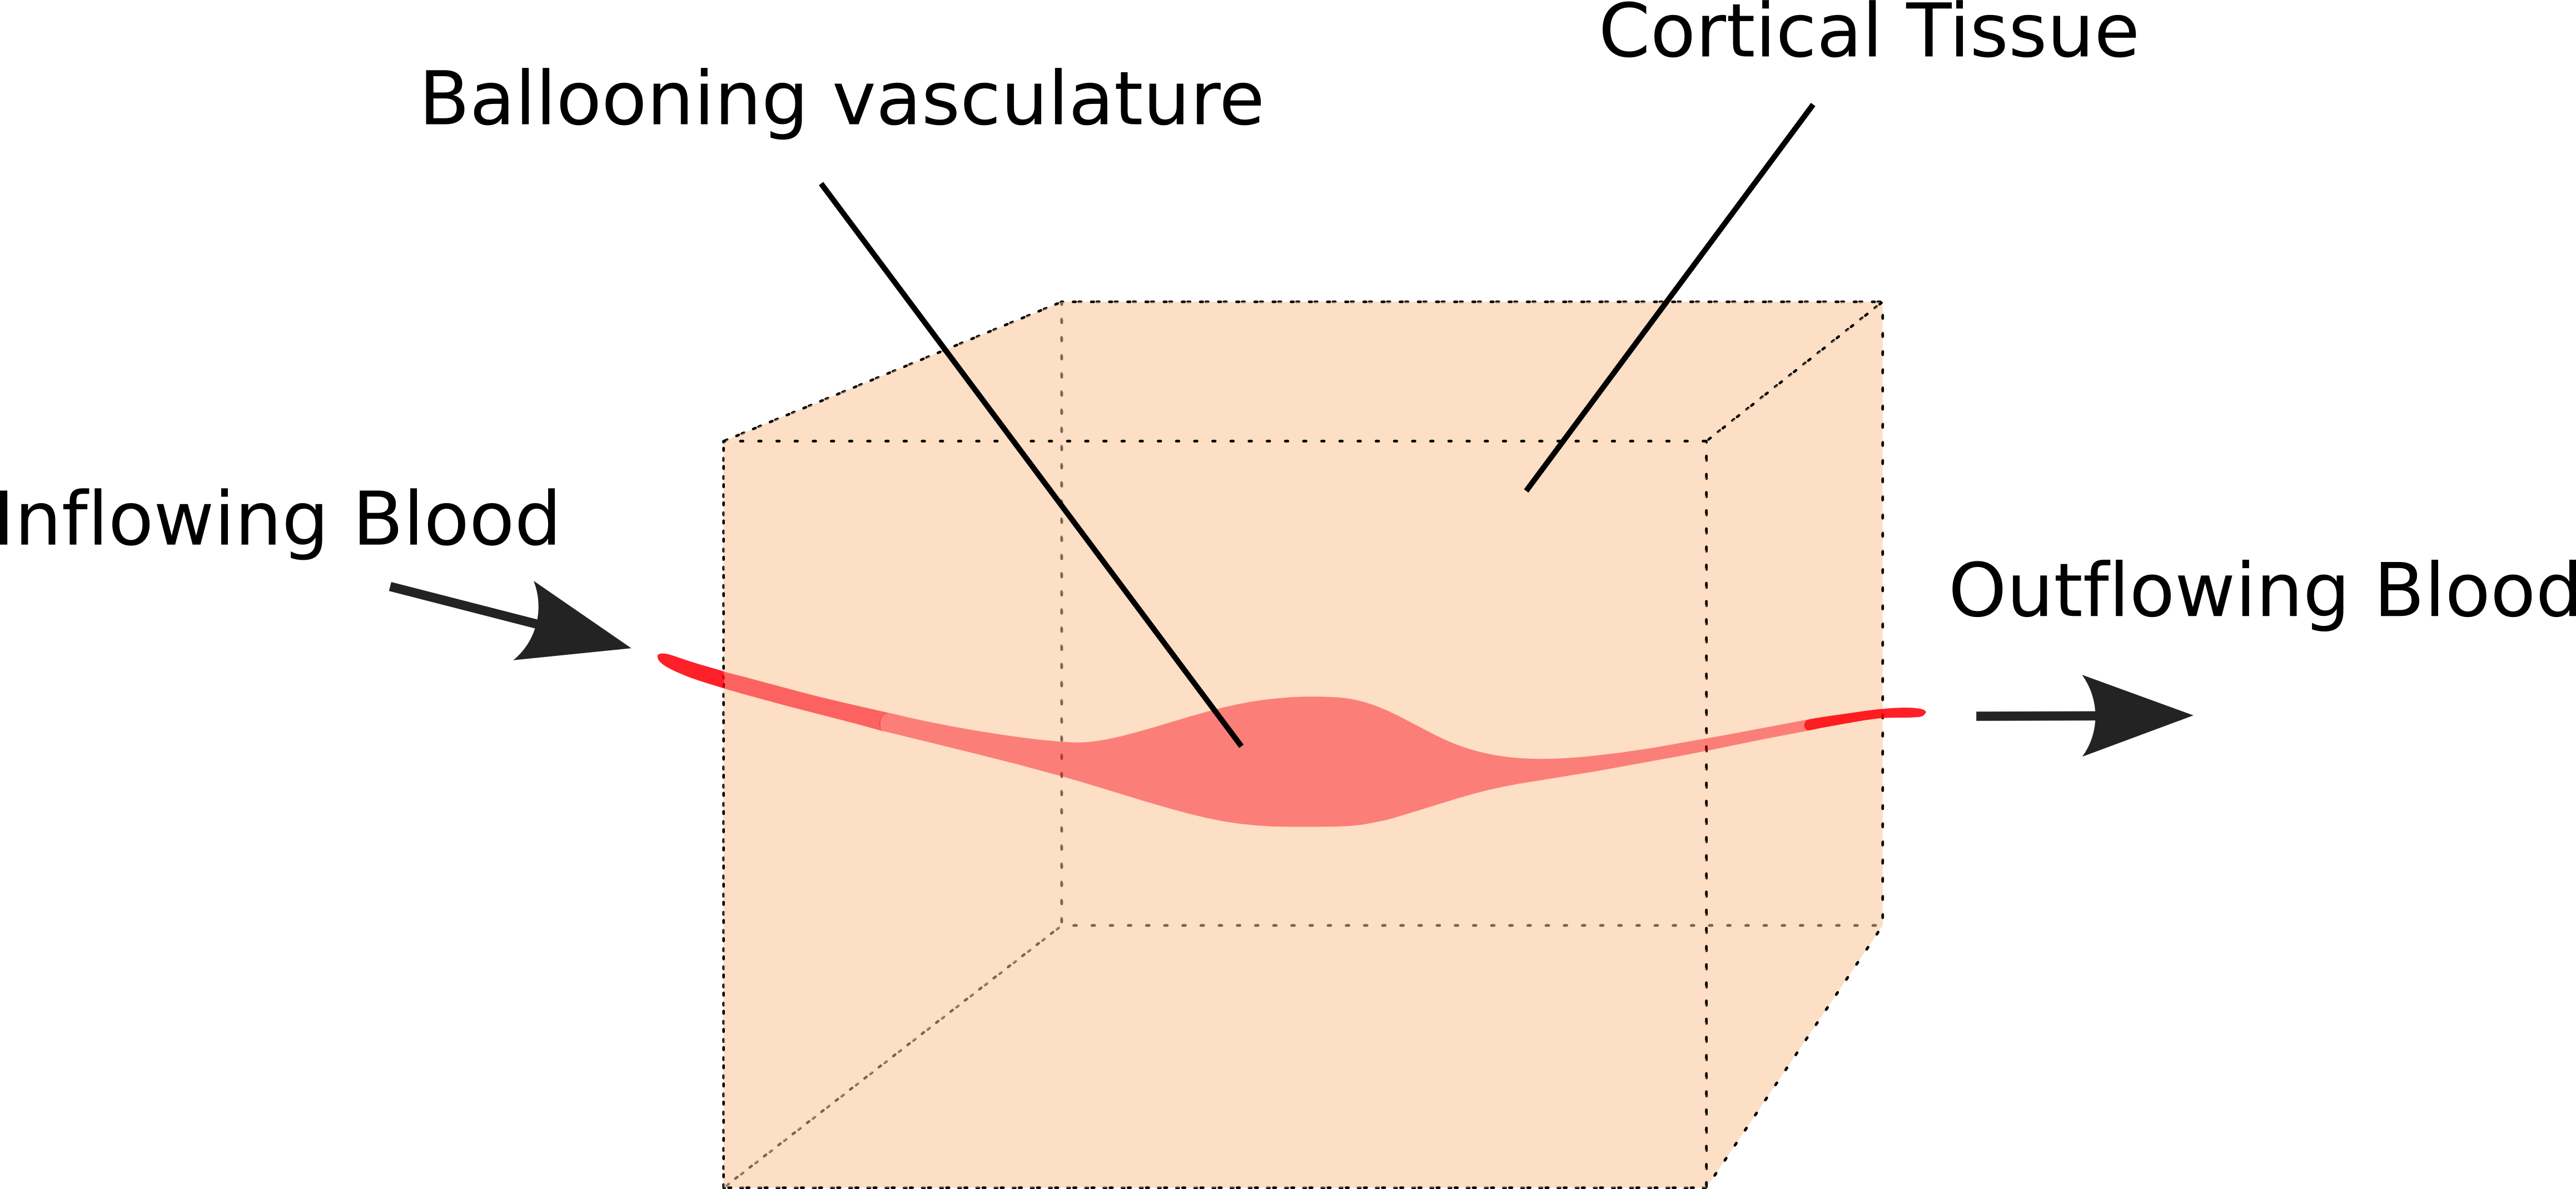
\includegraphics[width=\linewidth]{balloon-model-rastor}
  }
}

%%%%%%%%%%%%%%%%%%%%%%%%%%%%%%%%%%%%%%%%%%%%%%%%%%%%%%%%%%%%%%%
%%%%%  Previous Works
%%%%%%%%%%%%%%%%%%%%%%%%%%%%%%%%%%%%%%%%%%%%%%%%%%%%%%%%%%%%%%%

\frame{
\frametitle{1-D Penne's Bioheat Equation~\footlessfullcite{sotero2011}}
  \begin{align}
    C_{tissue} \frac{dT(t)}{dt} &= (\Delta H^{\circ}-\Delta H_{b}) CMRO_{2}\mid_{0} m(t) \nonumber \\
    &\quad {} - \rho_{b} C_{b} CBF\mid_{0} f(t) (T(t) - T_{a}) \nonumber \\
    &\qquad {} - \frac{C_{t}}{\tau} (T(t)-T_{0}) \nonumber
  \end{align}
  \medskip
  \small{
  \begin{align}    
    heat\ capacity\ &*\ change\ in\ temperature\ =\ heat\ generated\ by\ metabolism \nonumber \\
    &\quad  {} -\ heat\ lost\ due\ to\ convection \nonumber \\
    &\qquad {} -\ heat\ lost\ due\ to\ conduction \nonumber
  \end{align}
  }
}

%%%%%%%%%%%%%%%%%%%%%%%%%%%%%%%%%%%%%%%%%%%%%%%%%%%%%%%%%%%%%%%
%%%%%  Our Approach 
%%%%%%%%%%%%%%%%%%%%%%%%%%%%%%%%%%%%%%%%%%%%%%%%%%%%%%%%%%%%%%%


\frame{
\frametitle{Calculations Procedure}
  \centering
  \resizebox{\textwidth}{!}{%
    \tikzstyle{data} = [draw=none, fill=goldfish]
\tikzstyle{temptools} = [draw=none, fill=aoi]
\tikzstyle{spm} = [draw=none, fill=beachstorm]
\tikzstyle{params} = [draw=none, fill=pondwater]
\tikzstyle{line} = [draw, very thick, color=black!50, -stealth']

\begin{tikzpicture}[node distance=0.7cm, rectangle, text width=4.5cm, text badly centered, rounded corners, minimum height=1cm, anchor=north]     
  % Left column
    \node[data](fmridata){fMRI BOLD Data};
    \node[temptools, below=of fmridata](calcrest){Calculate resting state (avg\_NII\_rest)};
    \node[temptools, below=of calcrest](normalize){Normalize the data to resting state (avg\_NII\_normalize)};
    \node[temptools, below=of normalize](boldtomf){Calculate the change in metabolism and blood flow (BOLDtoMF)};
    % middle column
    \node[data, right=of fmridata](t1contrast){T1 contrast image};
    \node[spm, below=of t1contrast](segment){Segment image (SPM8)};
    \node[temptools, right=of boldtomf](buildhead){Build head matrix (ImportSegmentedT1)};
    % right column
    \node[temptools, right=of buildhead](calcequil){Calculate equilibrium temperature (tempCalcEquilibrium)};
    \node[params, above=of calcequil, xshift=-2cm](tissueparams){Tissue-specific parameters};
    % bottom
    \node[temptools, below=of buildhead, text width=8cm](calctemp){Find temperature change during activity (tempCalcDynMF)};
  
  \path[line](fmridata) -- (calcrest);
  \path[line](calcrest) -- (normalize);
  \path[line](normalize) -- (boldtomf);
  \path[line](t1contrast) -- (segment);
  \path[line](segment) -- (buildhead);
  \path[line](buildhead) -- (calcequil);
  \path[line](boldtomf) |- (calctemp);
  \path[line](buildhead) -- (calctemp);
  \path[line](calcequil) |- (calctemp); 
  \path[line](tissueparams) -| (buildhead);
\end{tikzpicture}
  }
}

\frame{
\frametitle{3-D Penne's Bioheat Equation~\footlessfullcite{collins}}
  \begin{equation*}
  	\rho c \frac{dT}{dt} = k \nabla^{2}T-\rho_{blood}f(t)wc_{blood}(T-T_{blood})+m(t)Q_{m} 
  \end{equation*}
}

\frame{
\frametitle{The Segmented Head}
  \centering
  \hspace{2cm}
  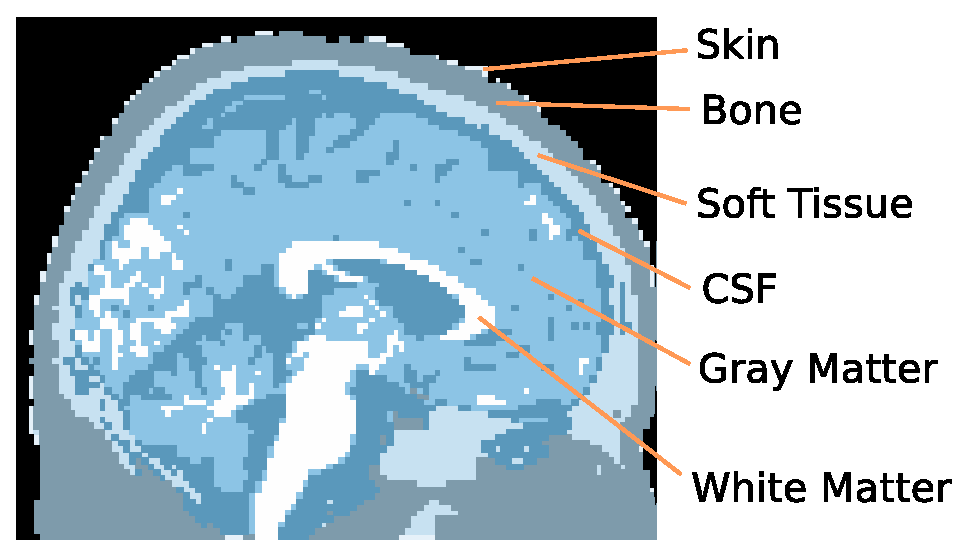
\includegraphics[width=0.7\textwidth]{segmented-head}
  \medskip
  \tiny{
  \begin{tabular*}{17cm}{@{} l p{2.5cm}p{2cm}p{2.5cm}p{2.5cm}p{2cm}l@{}}
	  \toprule
	  Tissue & $f_0$ \newline $100 \; ml/(g \; min)$ & $\rho$ \newline $kg/m^{3}$ & $c$ \newline $J \: kg^{-1} \: {}^\circ C^{-1}$ & $k$ \newline $W \: m^{-1} \: {}^\circ C^{-1}$ & $Q_{m}$ \newline $W/m^{3}$ \\
	  \midrule
		Bone & 3 & 1,080 & 2,110 & 0.65 & 26.1 \\
		Cerebrospinal Fluid & 0 & 1,007 & 3,800 & 0.50 & 0 \\
		Gray Matter & 67.1 & 1,035.5 & 3,680 & 0.565 & 15,575 \\
		White Matter & 23.7 & 1,027.4 & 3,600 & 0.503 & 5,192 \\
		Muscle & 3.8 & 1,041 & 3,720 & 0.4975 & 687 \\
		Skin & 12 & 1,100 & 3,150 & 0.342 & 1,100 \\
		\bottomrule
	\end{tabular*}
	}
}

\frame{
\frametitle{Equilibrium Temperature}
\centering
\begin{columns}
  \begin{column}{0.5\textwidth}
    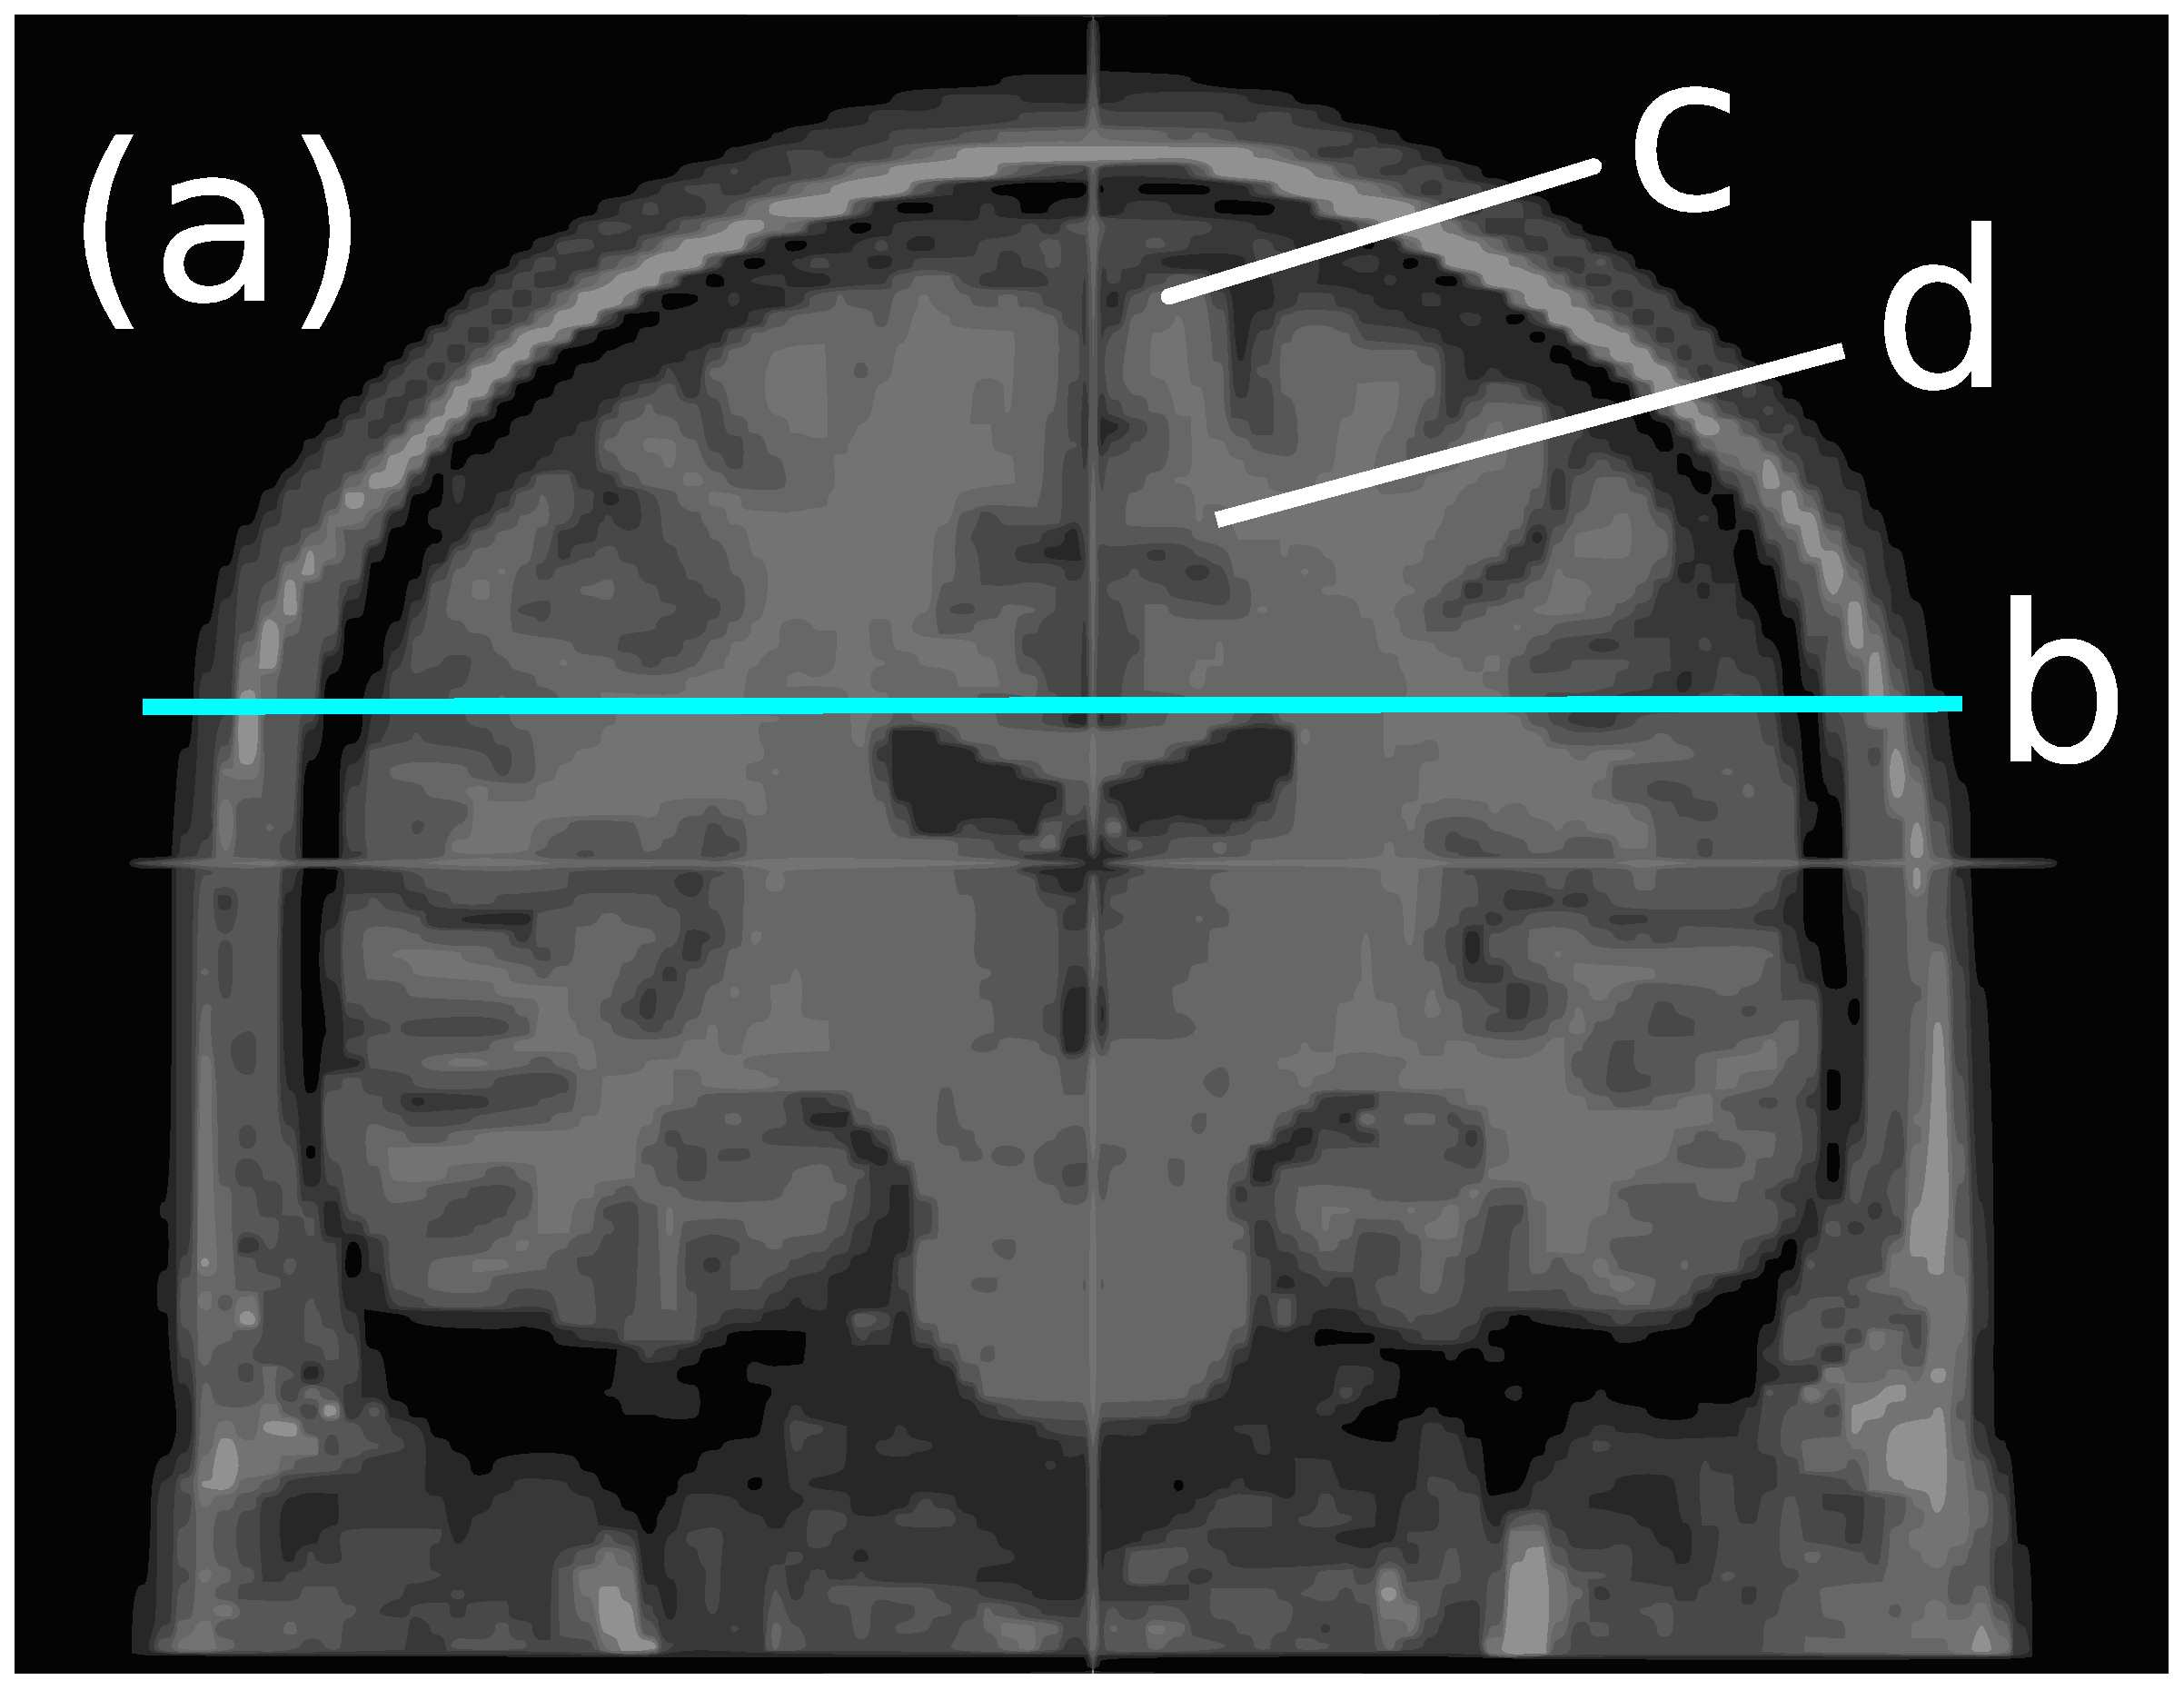
\includegraphics[width=\textwidth]{headref}
  \end{column}
  \begin{column}{0.5\textwidth}
    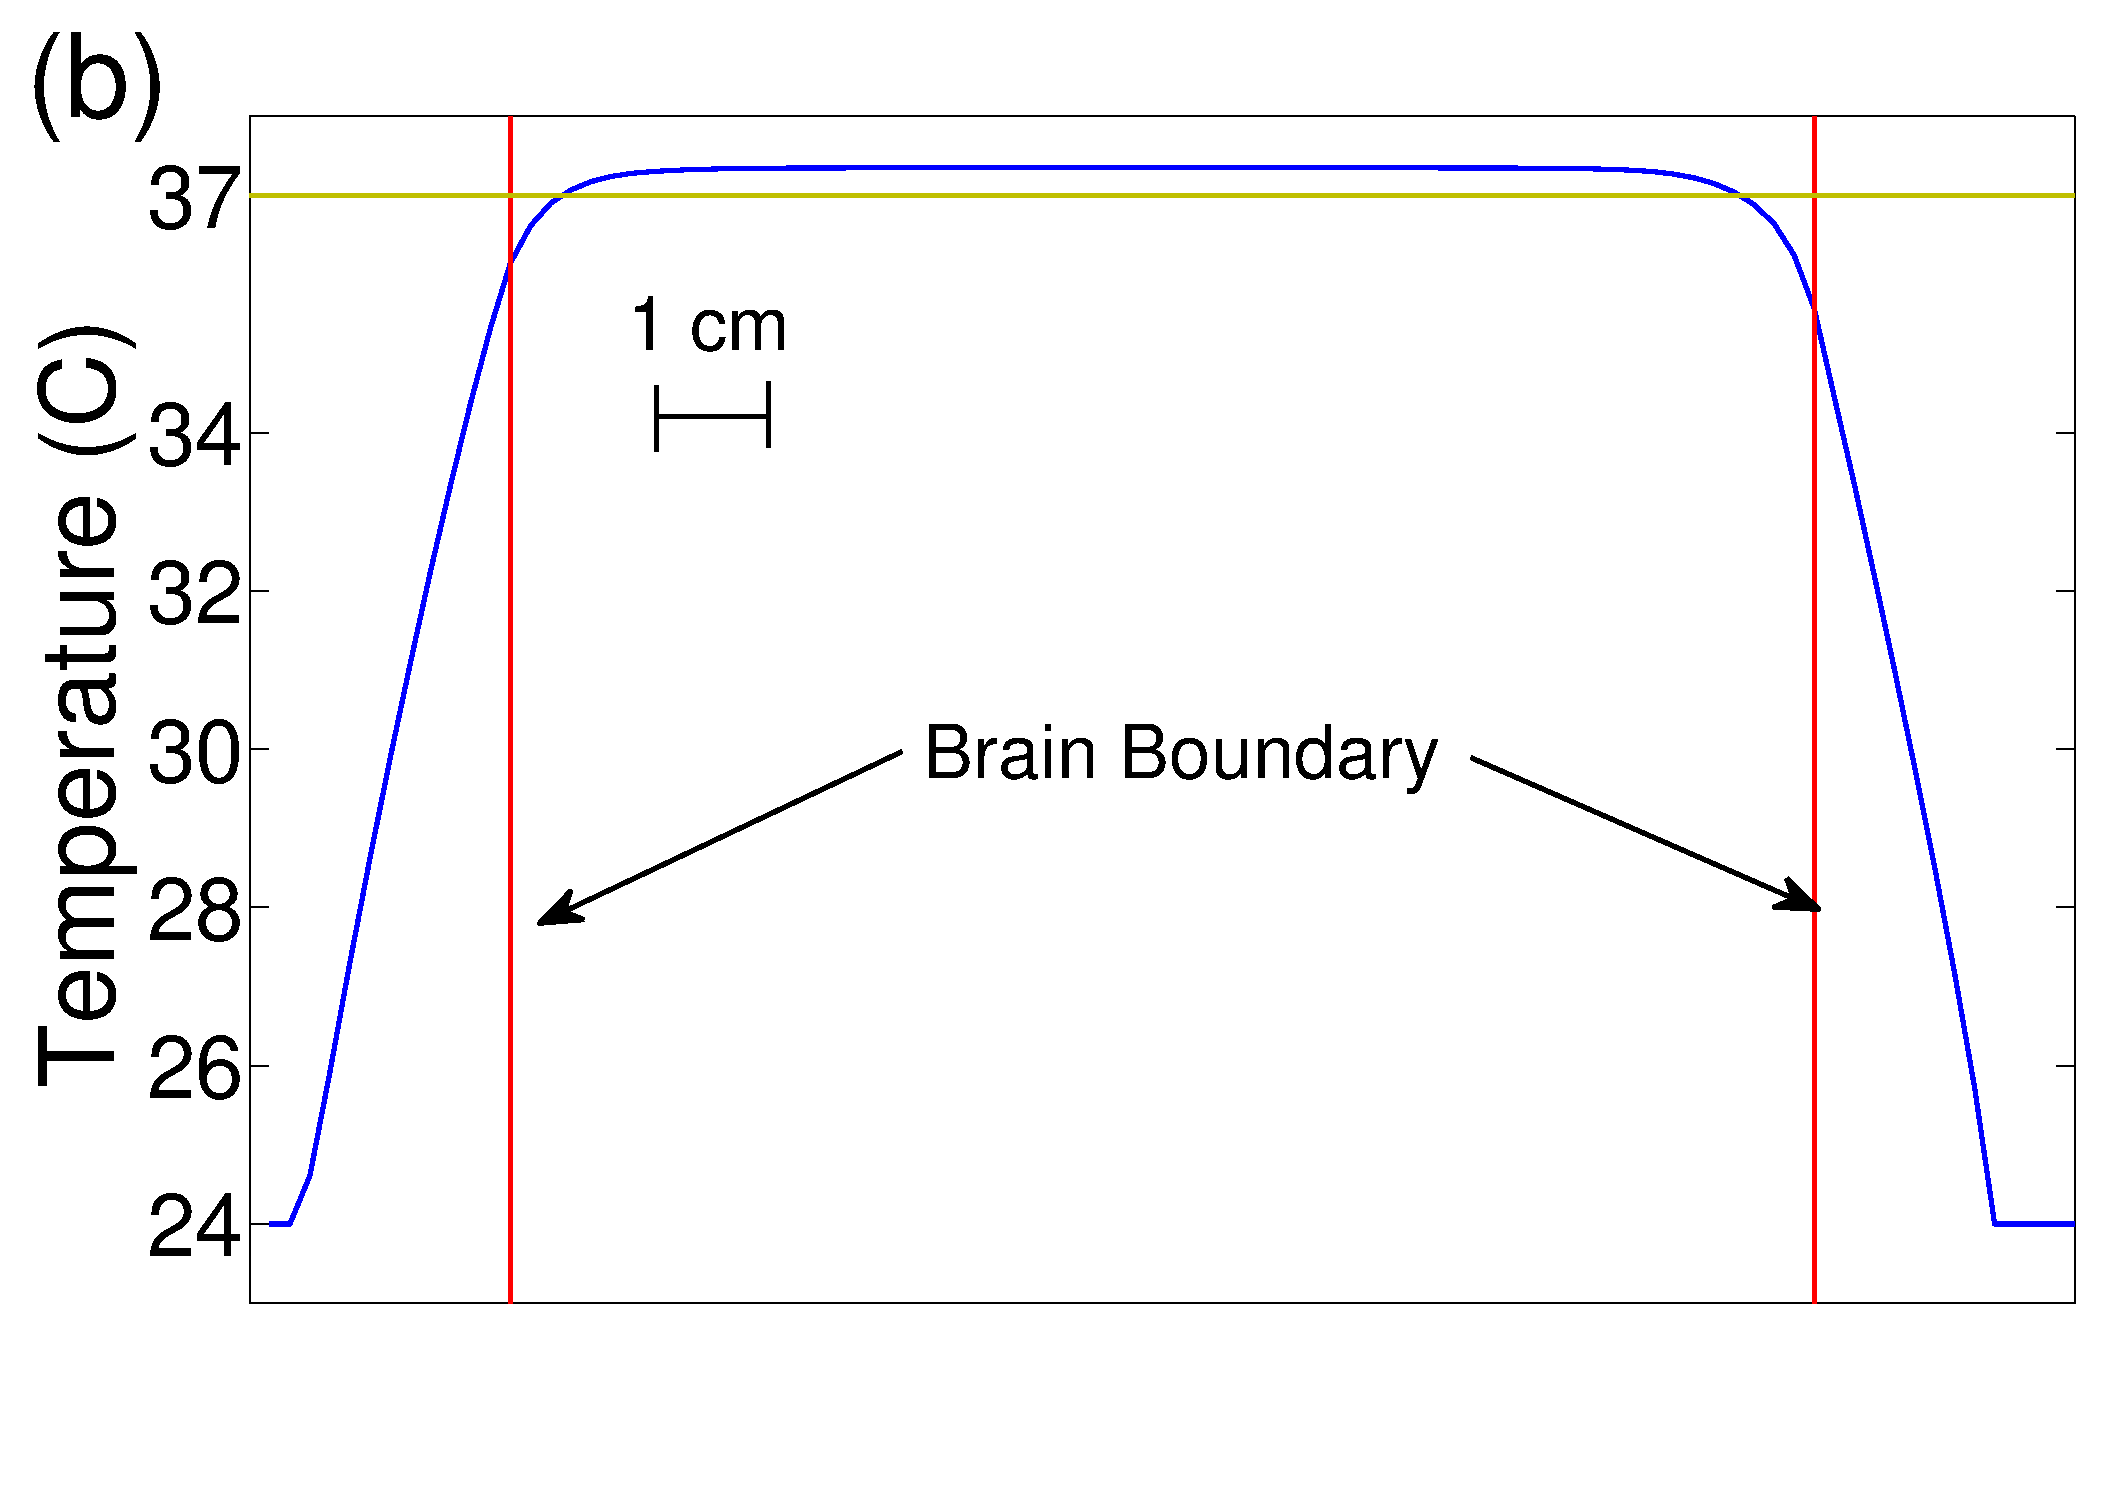
\includegraphics[width=\textwidth] {equilibrium_temperature_0_55_52} 
  \end{column}
\end{columns}
}

\frame{
\frametitle{Synthetic BOLD}
  \resizebox{\textwidth}{!}{
  \begin{tabular}{c}
    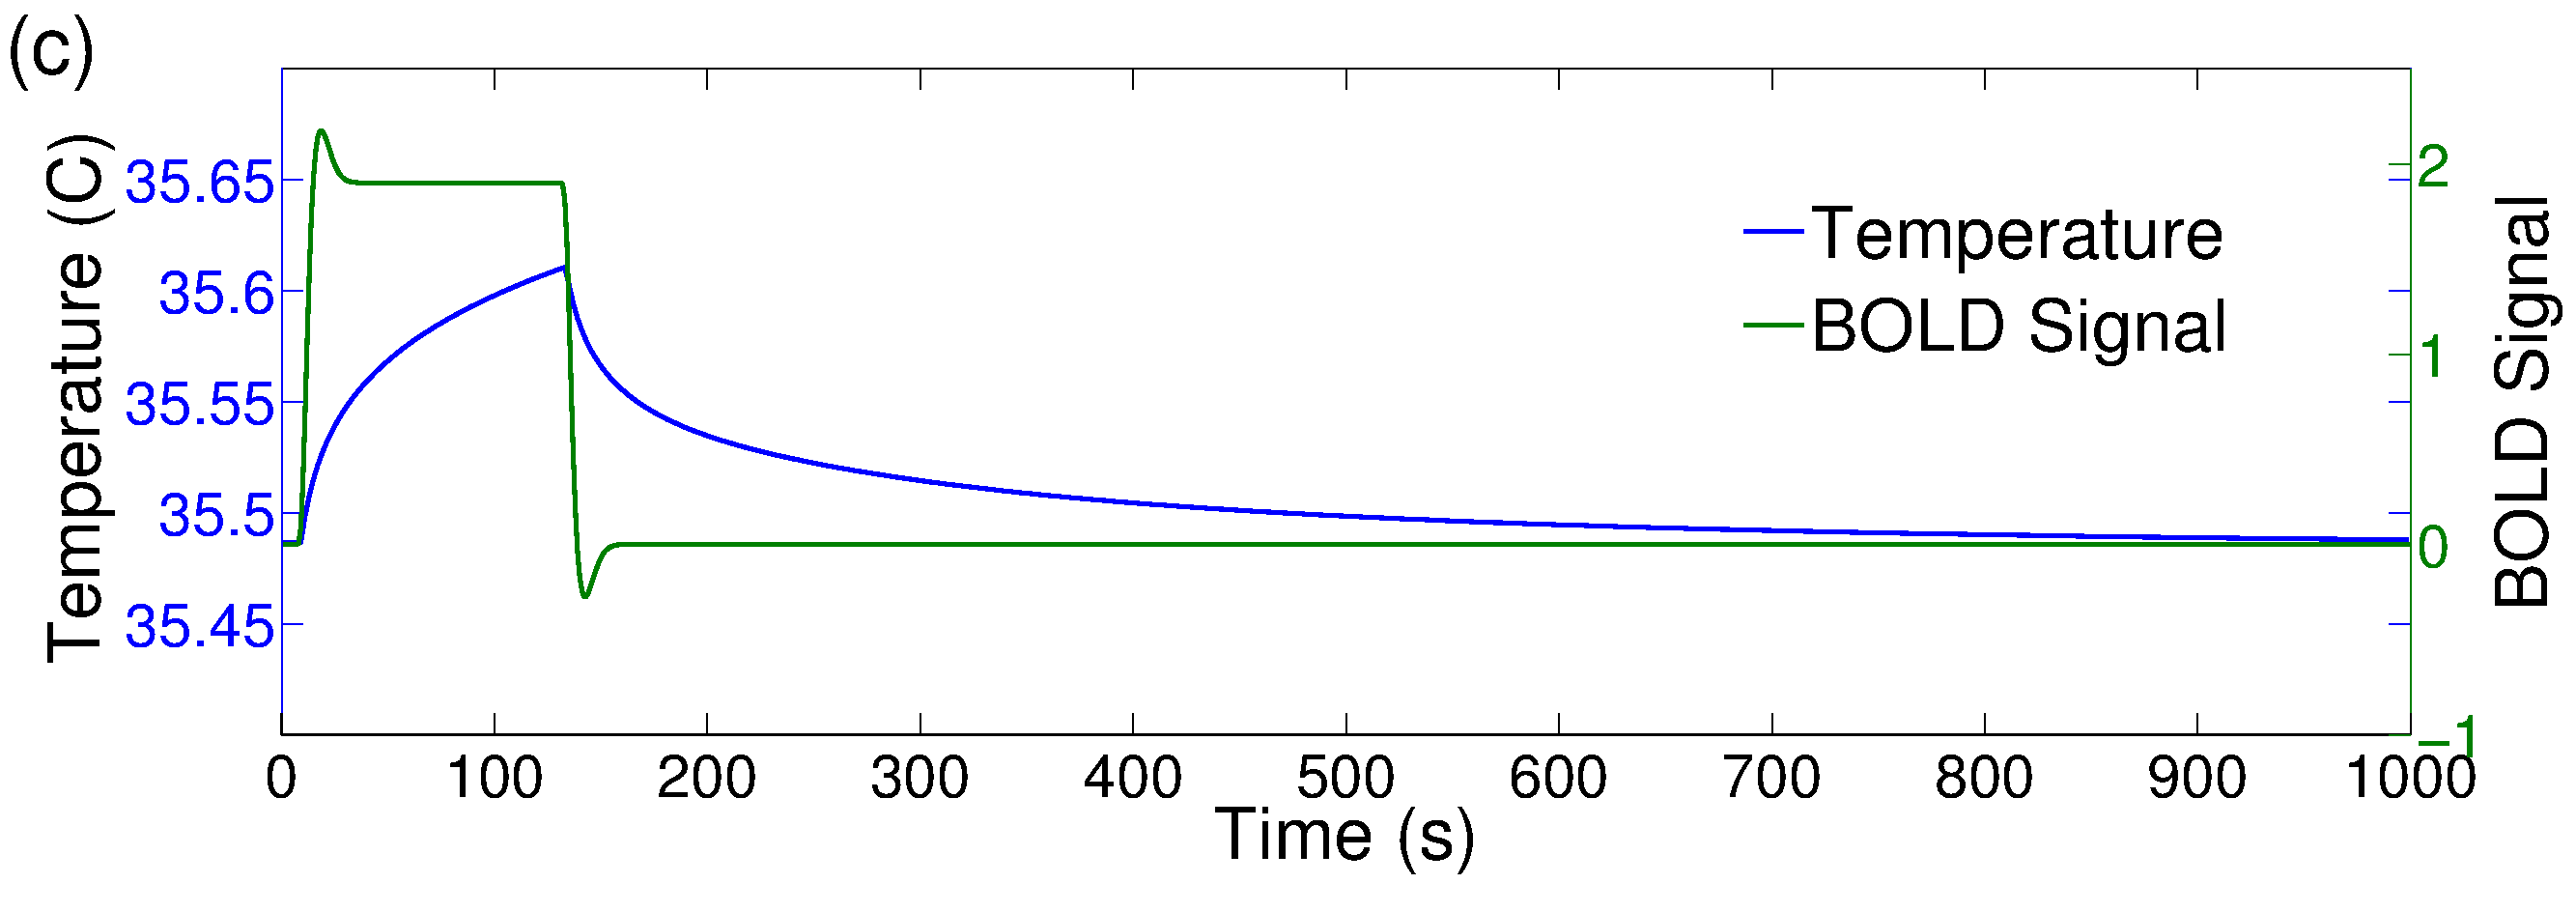
\includegraphics{sim_bold_(48_58_76)} \\
    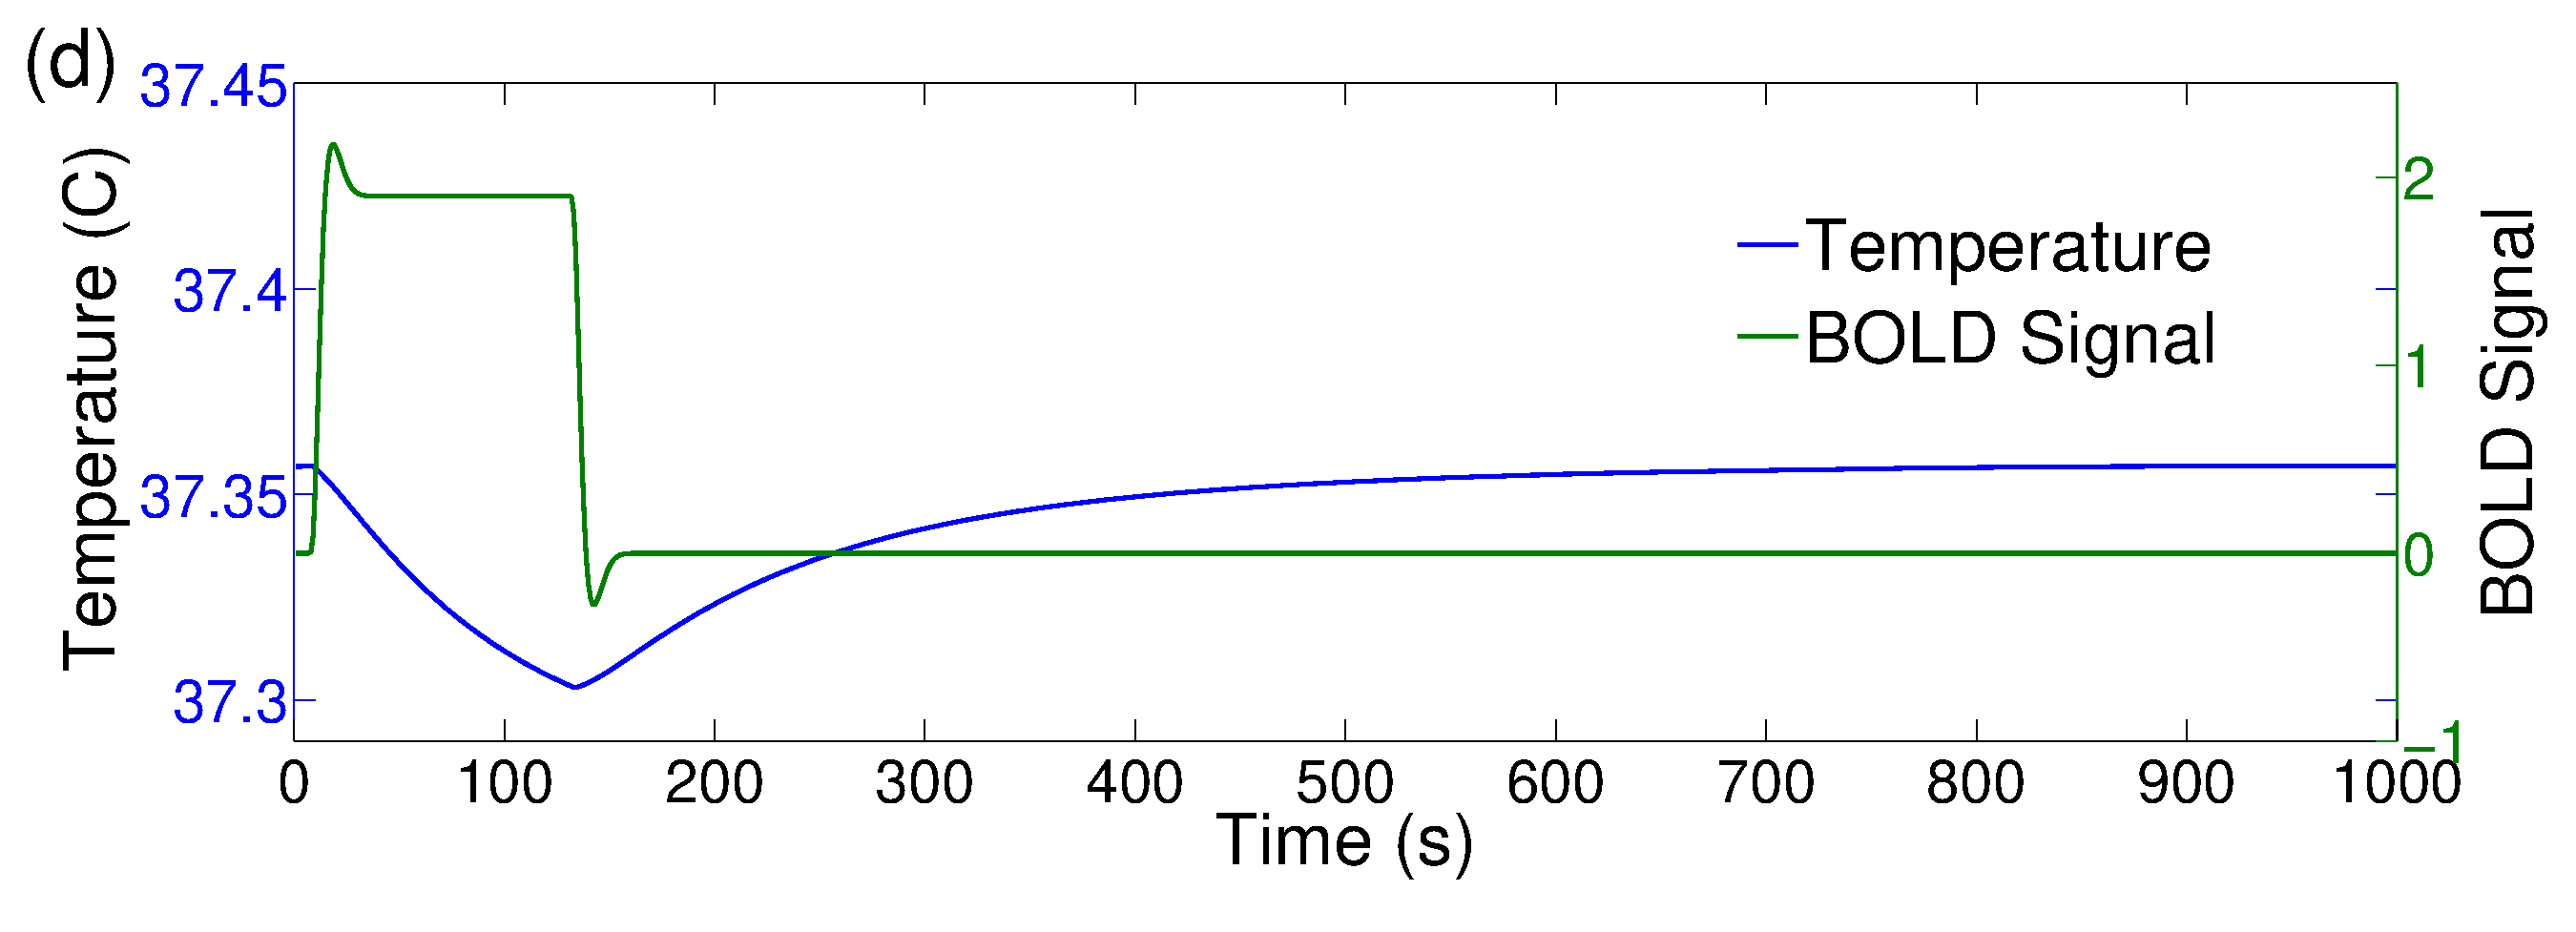
\includegraphics{sim_bold_(48_58_56)}
  \end{tabular}
  }
}

\frame{
\frametitle{Experimental BOLD Data}
  \begin{columns}
    \begin{column}{0.5\textwidth}
      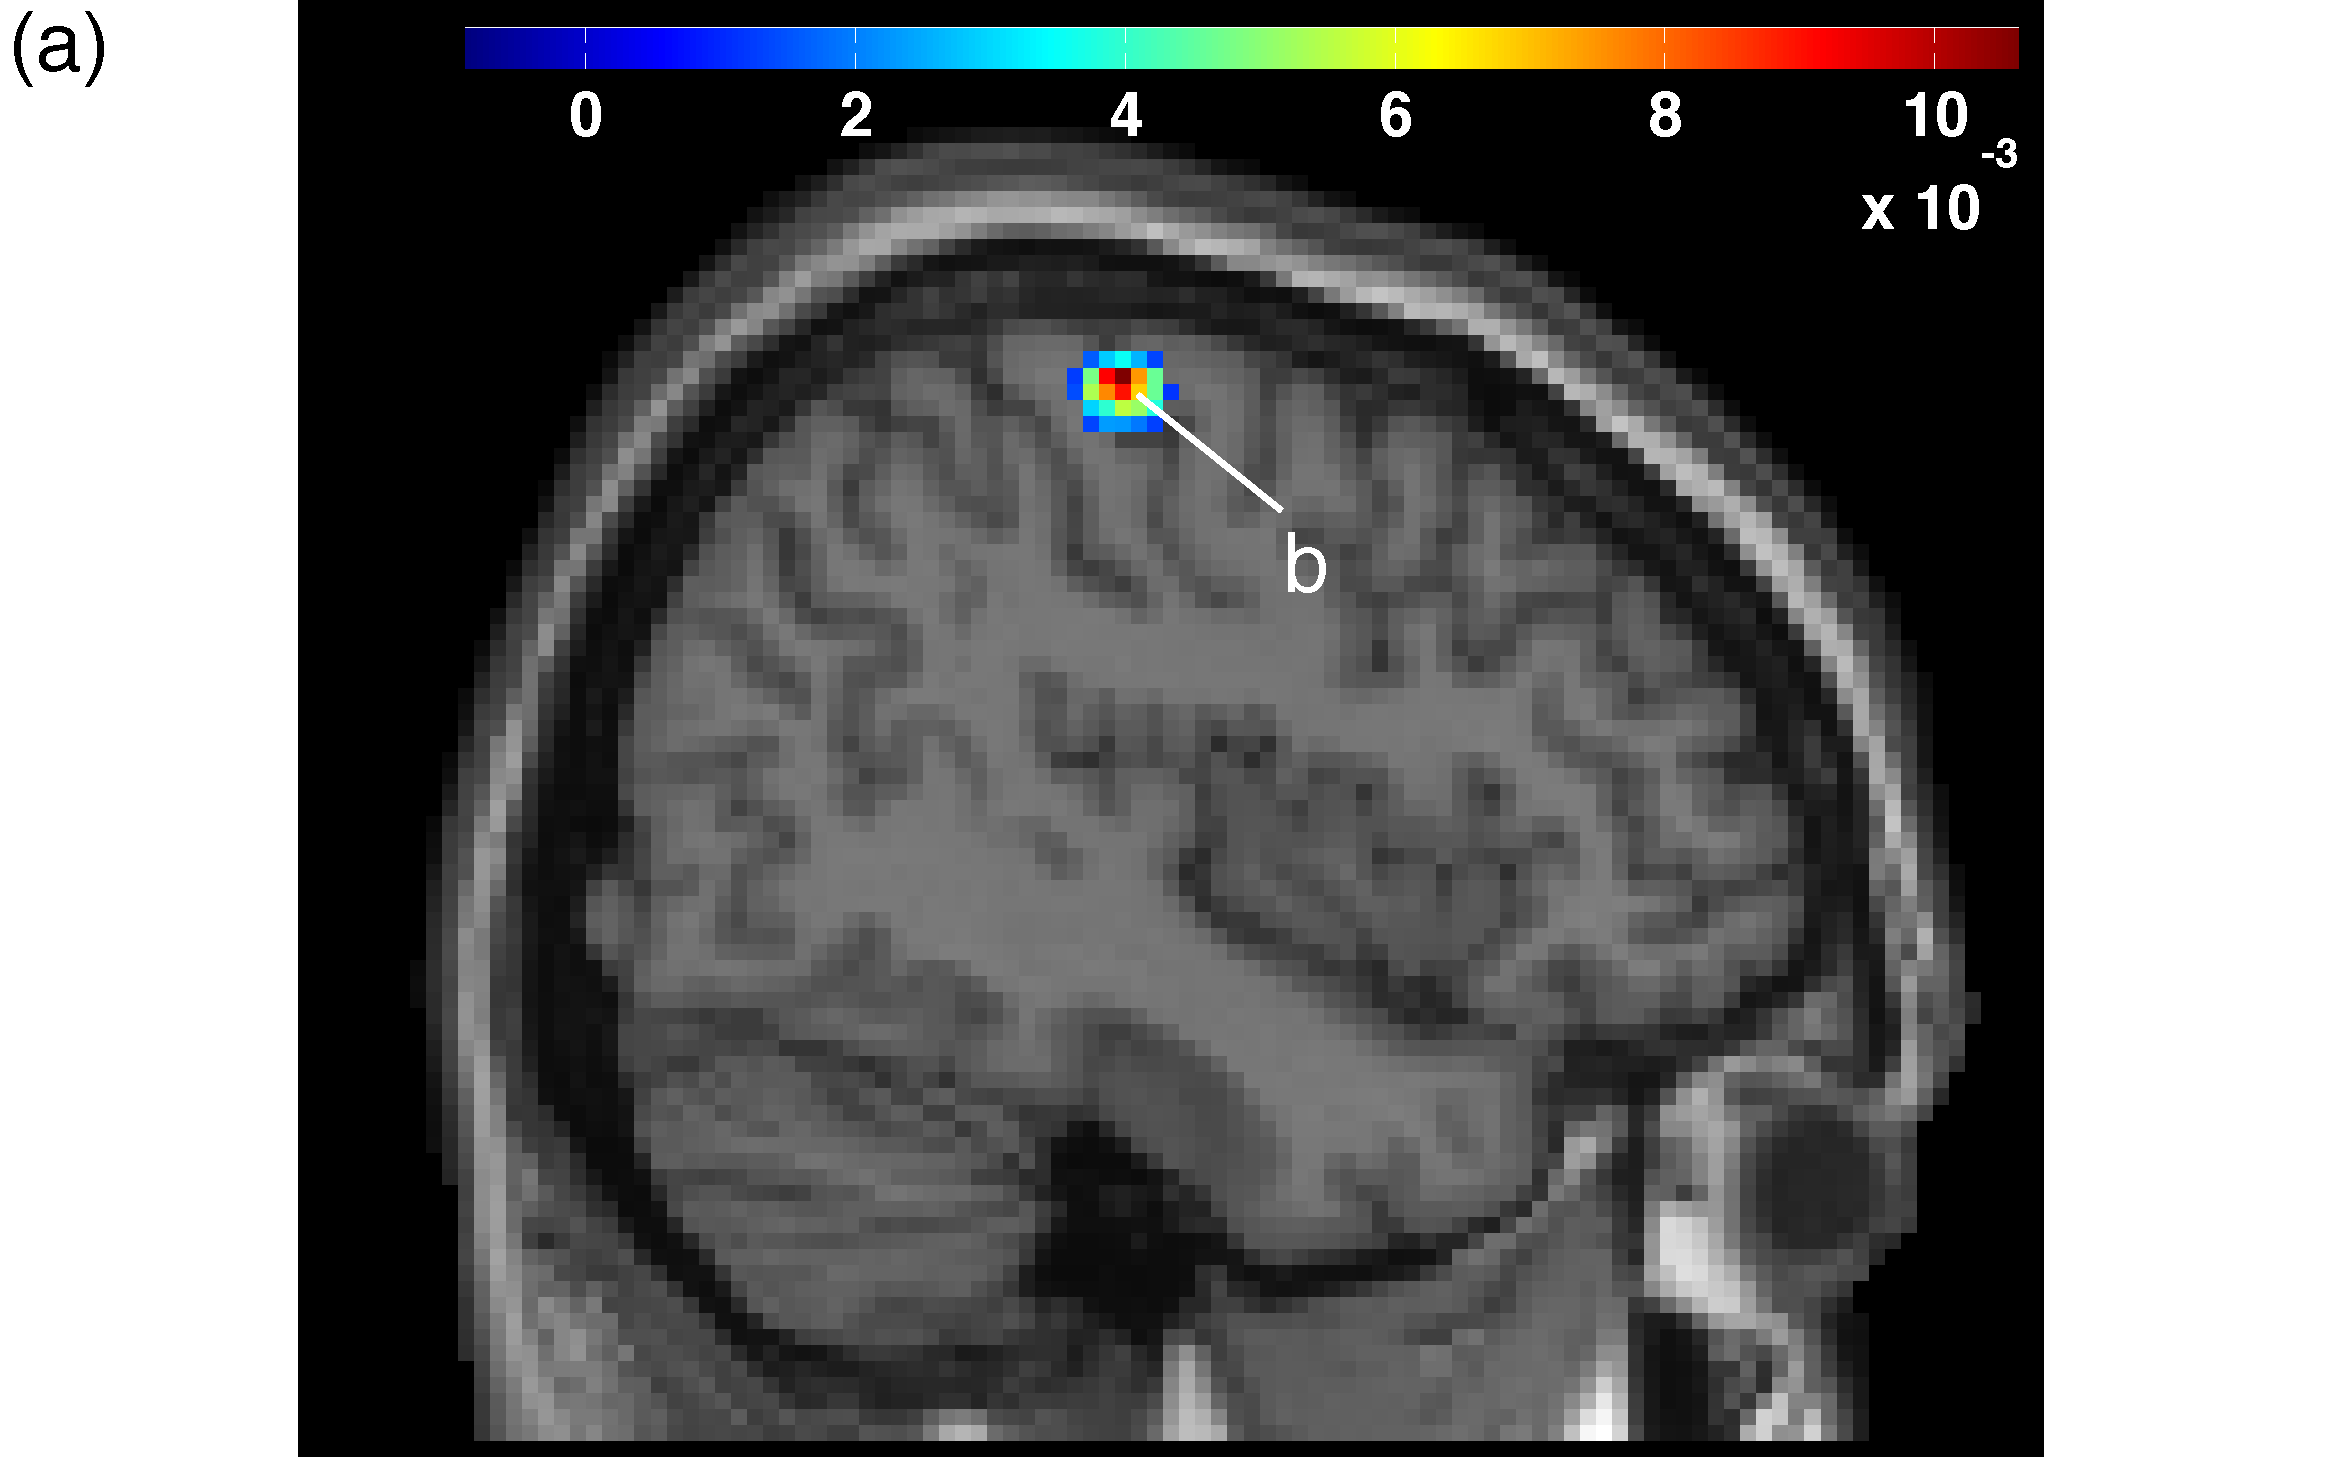
\includegraphics[width=\textwidth]{slice_x_24}
    \end{column}
    \begin{column}{0.5\textwidth}
      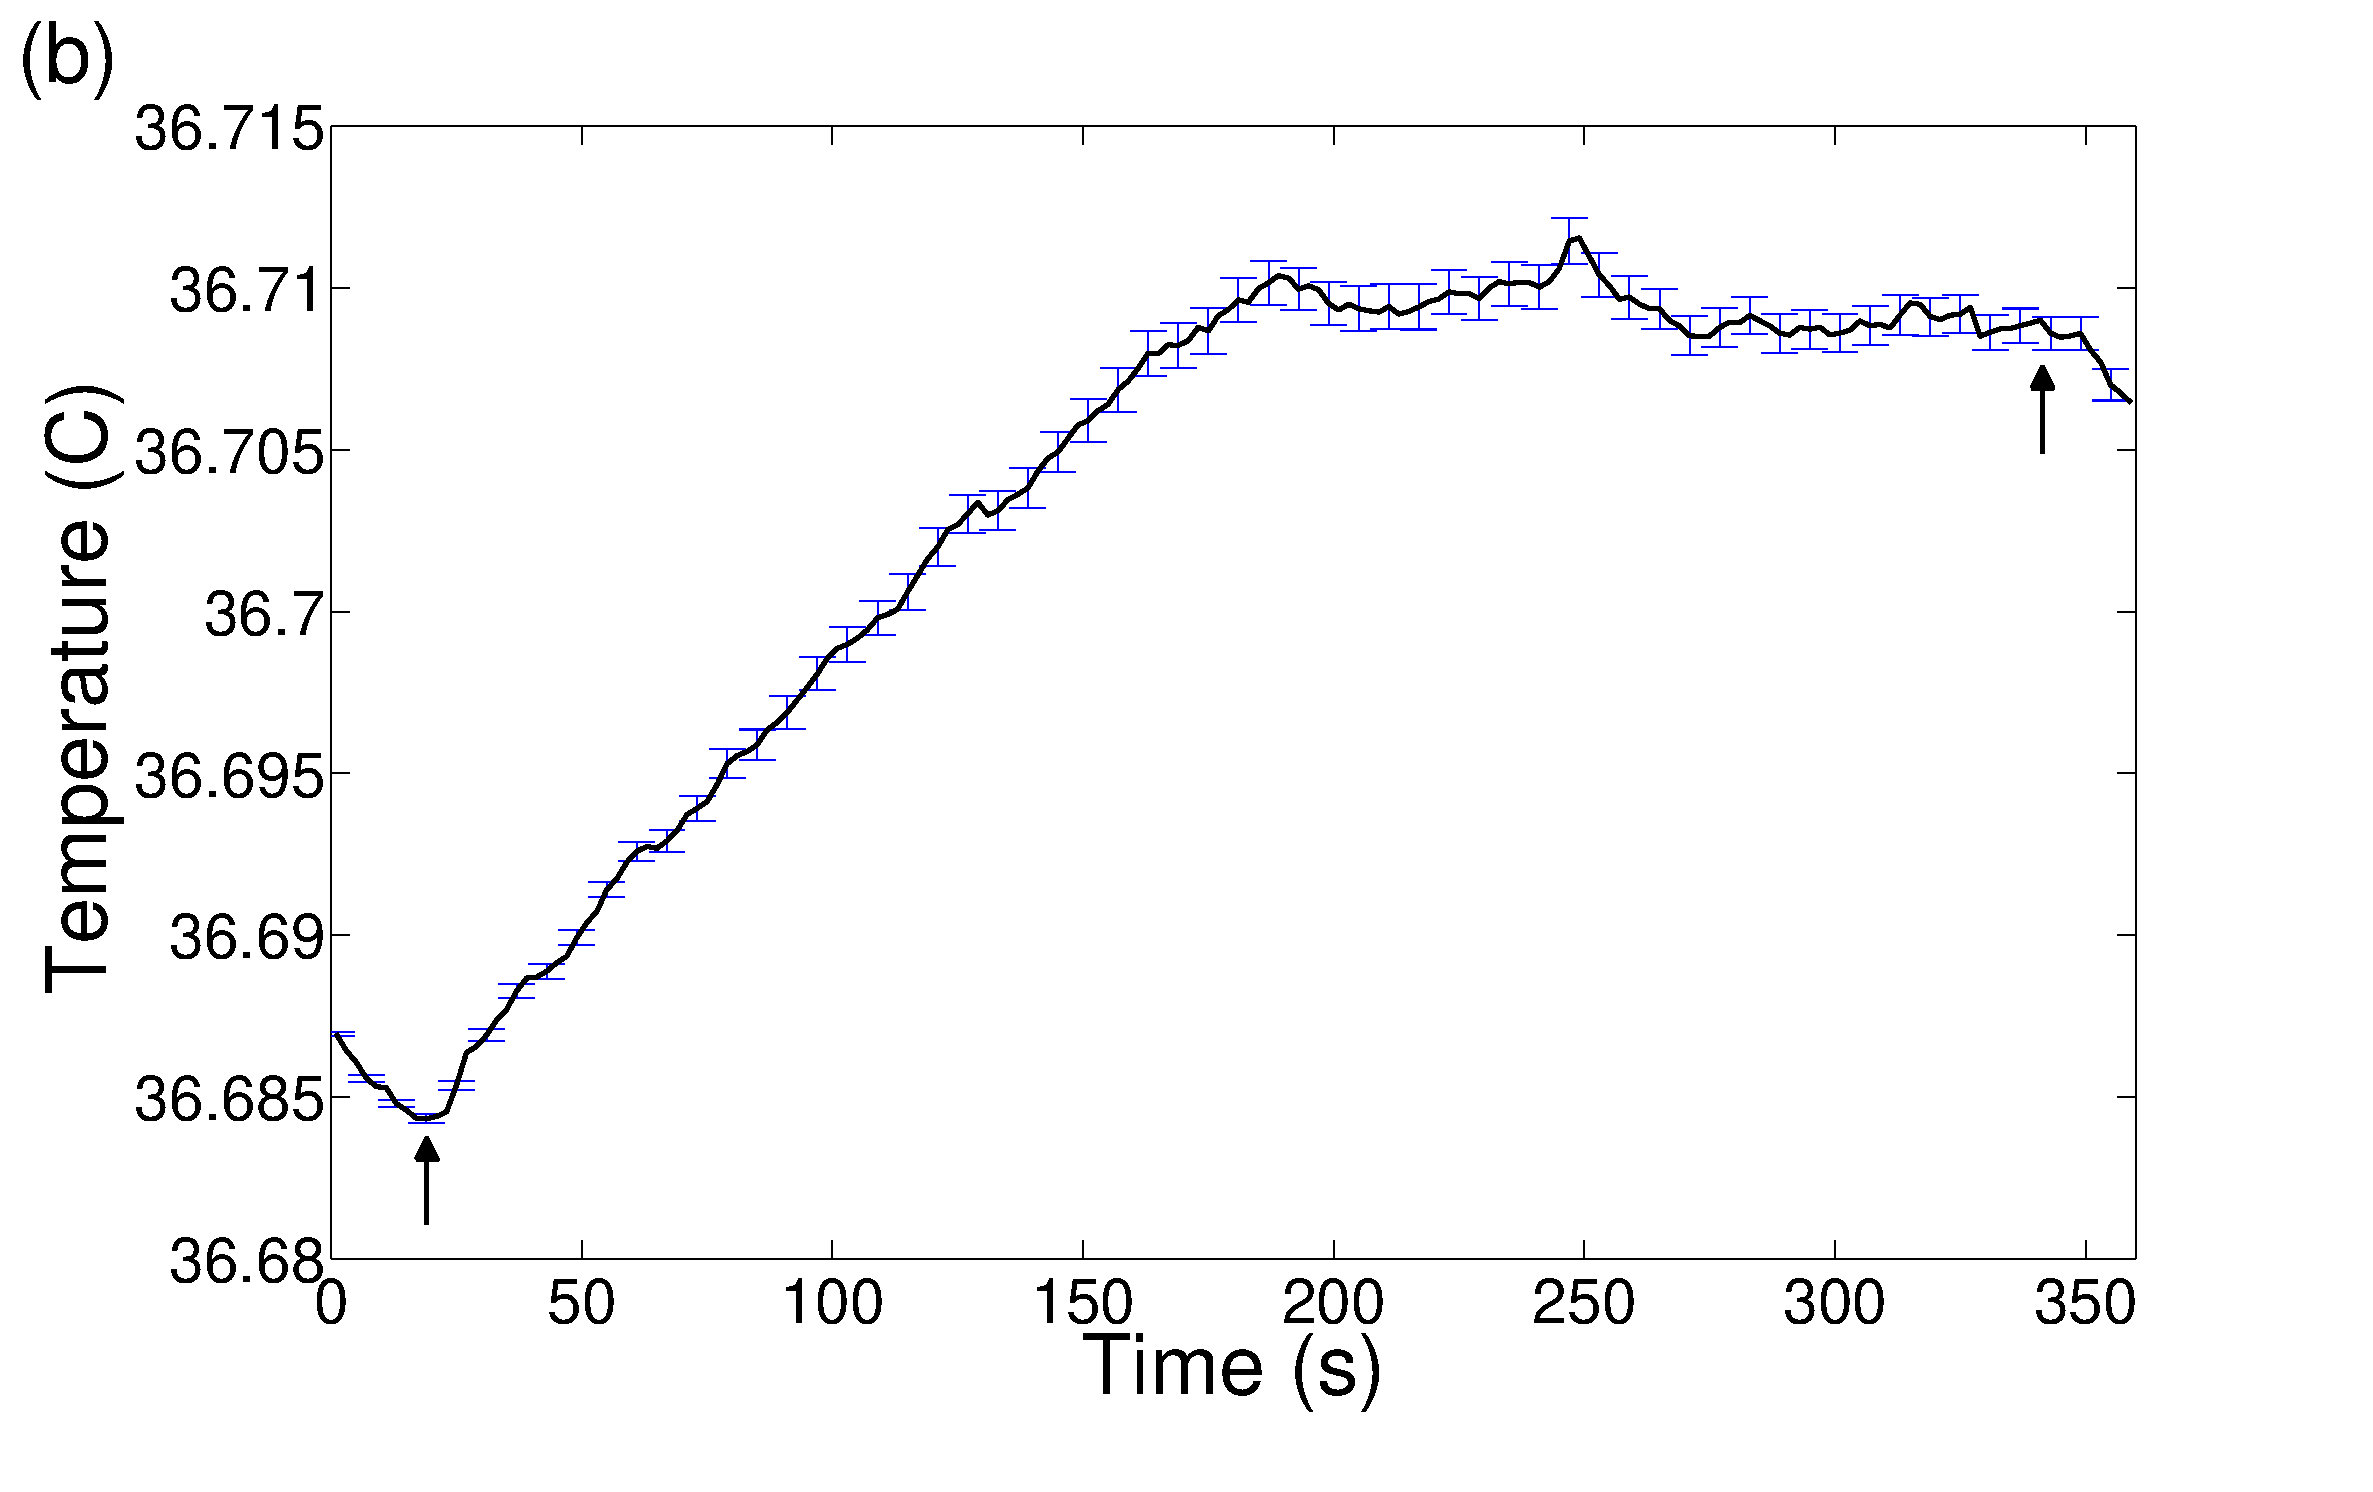
\includegraphics[width=\textwidth]{avg_data_24_52_67}
    \end{column}
  \end{columns}
}

%%%%%%%%%%%%%%%%%%%%%%%%%%%%%%%%%%%%%%%%%%%%%%%%%%%%%%%%%%%%%%%
%%%%%  Optical Techniques
%%%%%%%%%%%%%%%%%%%%%%%%%%%%%%%%%%%%%%%%%%%%%%%%%%%%%%%%%%%%%%%

\frame{
\frametitle{fMRI vs. fNIR}
  \scriptsize{
  \renewcommand{\arraystretch}{2}
  \begin{tabularx}{\linewidth}{lp{3cm}p{3cm}}
    \toprule
                         & fMRI             & fNIR            \\
    \midrule
    Spatial Resolution   & 8--27 mm$^3$  & $\sim$ 1--10 cm$^3$ \\
    Temporal Resolution  & 1--2 s        & $\sim$ 10$^{-3}$ s \\
    Measurement Parameter& blood volume, flow, and O$_2$ metabolism & oxyHb and deoxyHb concentrations \\
    Motion               & Must Remain Stationary & Small movements OK \\
    Penetration          & Whole-head    & outer 2--4 mm of brain tissue \\
    \bottomrule
  \end{tabularx}
  }
}

\frame{
\frametitle{Near-infrared Absorption Spectra}
  \centering
  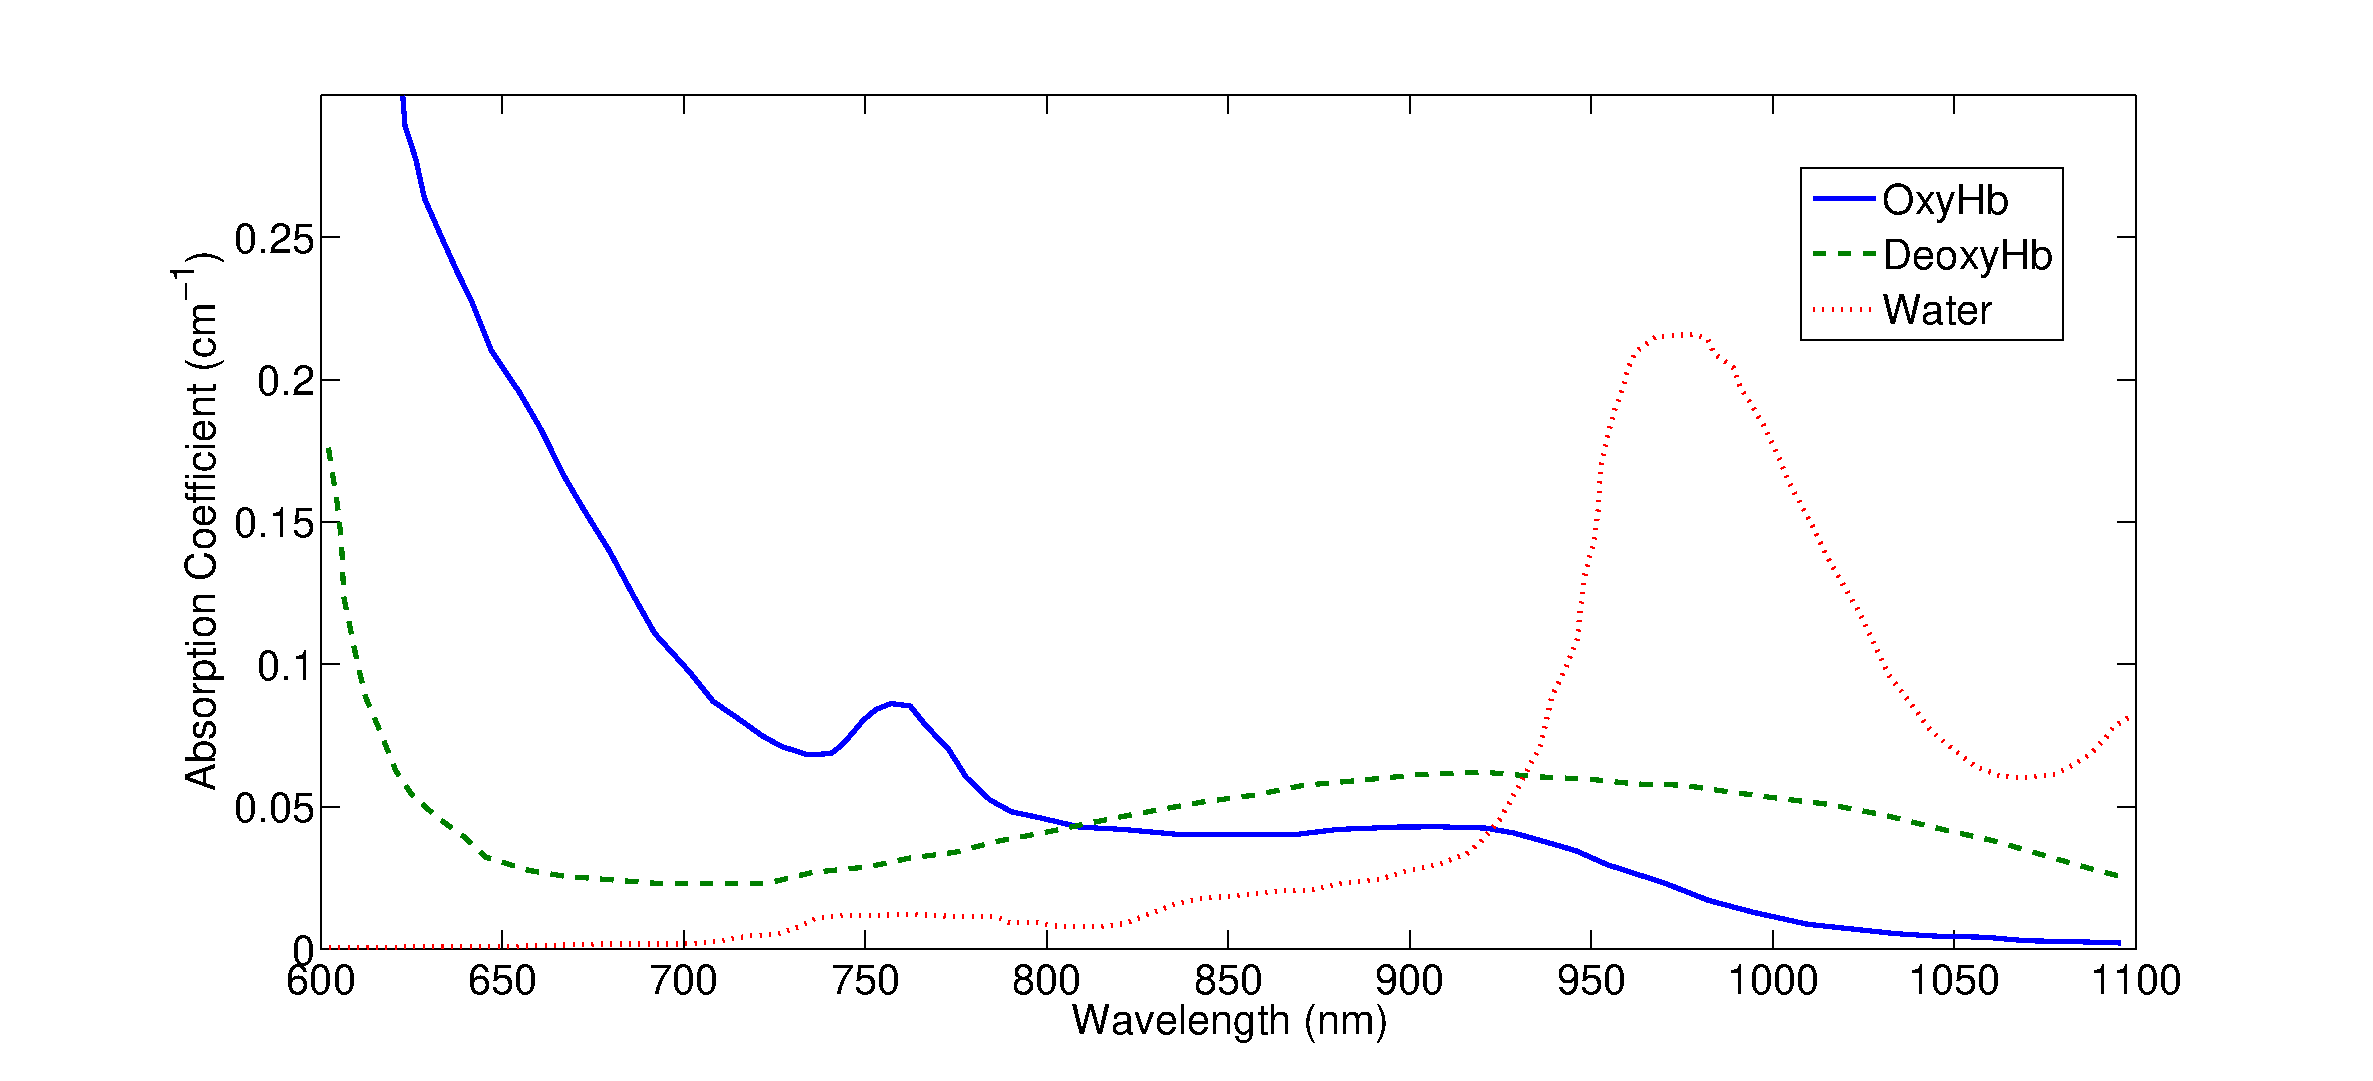
\includegraphics[width=\textwidth]{AbsorptionData}
}

\frame{
\frametitle{Typical fNIRS Setup}
  \centering
  \resizebox{\textwidth}{!}{
  \tikzstyle{detector} = [circle,draw, ultra thick, fill=blue!20]
\tikzstyle{ann} = [draw=none,fill=none,right]
\tikzstyle{led} = [star,star points=10,draw, thick, fill=red]
\tikzstyle{l} = [draw, very thick, color=black, dashed]
\tikzstyle{legend-box} = [rectangle, draw, thick, fill=none, minimum height=2cm, minimum width=3.5cm]
\begin{tikzpicture}
  \matrix[row sep=1.5cm,column sep=1.5cm] {
  \node[detector] (d11) {}; & &
  \node[detector] (d12) {}; & &
  \node[detector] (d13) {}; & &
  \node[detector] (d14) {}; \\
  & \node[led] (e1) {}; &
  & \node[led] (e2) {}; &
  & \node[led] (e3) {}; \\
  \node[detector] (d21) {}; & &
  \node[detector] (d22) {}; & &
  \node[detector] (d23) {}; & &
  \node[detector] (d24) {};\\
  };
  \node[ann, right=of d11, yshift=-1cm] {$l$};
  \node[detector, right=of d14, yshift=-1.2cm] (dRef) {};
  \node[led, below=of dRef, yshift=0.7cm]      (eRef) {};
  \node[ann, right=of dRef, xshift=-0.9cm] {Detector};
  \node[ann, right=of eRef, xshift=-0.9cm] {Emitter};
  \node[legend-box, right=of d14, yshift=-1.6cm, xshift=-0.5cm]{};
  \path[l](d11.south east) -- (e1.north west);
  \path[l](d12.south west) -- (e1.north east);
  \path[l](d12.south east) -- (e2.north west);
  \path[l](d13.south west) -- (e2.north east);
  \path[l](d13.south east) -- (e3.north west);
  \path[l](d14.south west) -- (e3.north east);
  \path[l](d21.north east) -- (e1.south west);
  \path[l](d22.north west) -- (e1.south east);
  \path[l](d22.north east) -- (e2.south west);
  \path[l](d23.north west) -- (e2.south east);
  \path[l](d23.north east) -- (e3.south west);
  \path[l](d24.north west) -- (e3.south east);
\end{tikzpicture}
  }
}

\frame{
\frametitle{fNIRS Penetration}
  \centering
  \includegraphics[width=\textwidth]{fnir-penetration}
}

\frame{
\frametitle{Black-body Emission}
  \begin{columns}
    \begin{column}{0.8\textwidth}
      \centering
      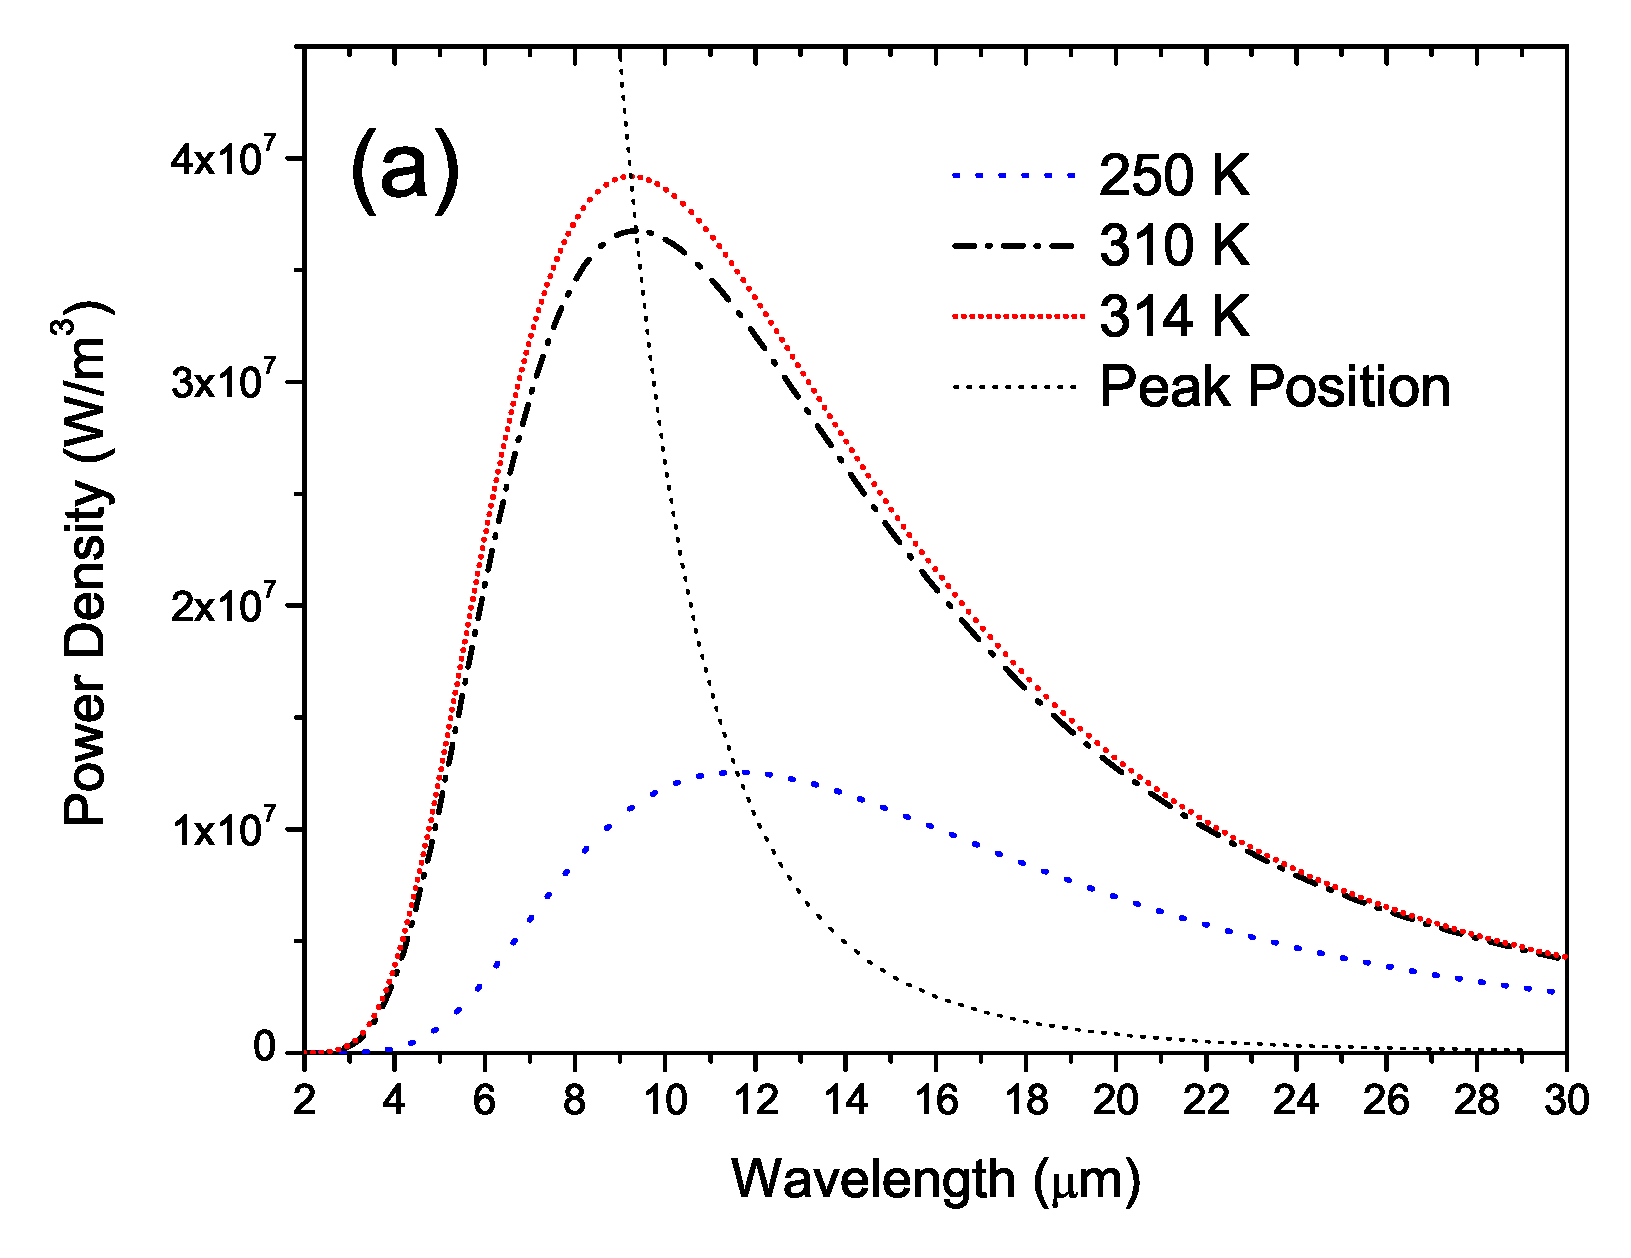
\includegraphics[width=\linewidth]{blackbody-1}
    \end{column}
    \begin{column}{0.2\textwidth}
      \centering
      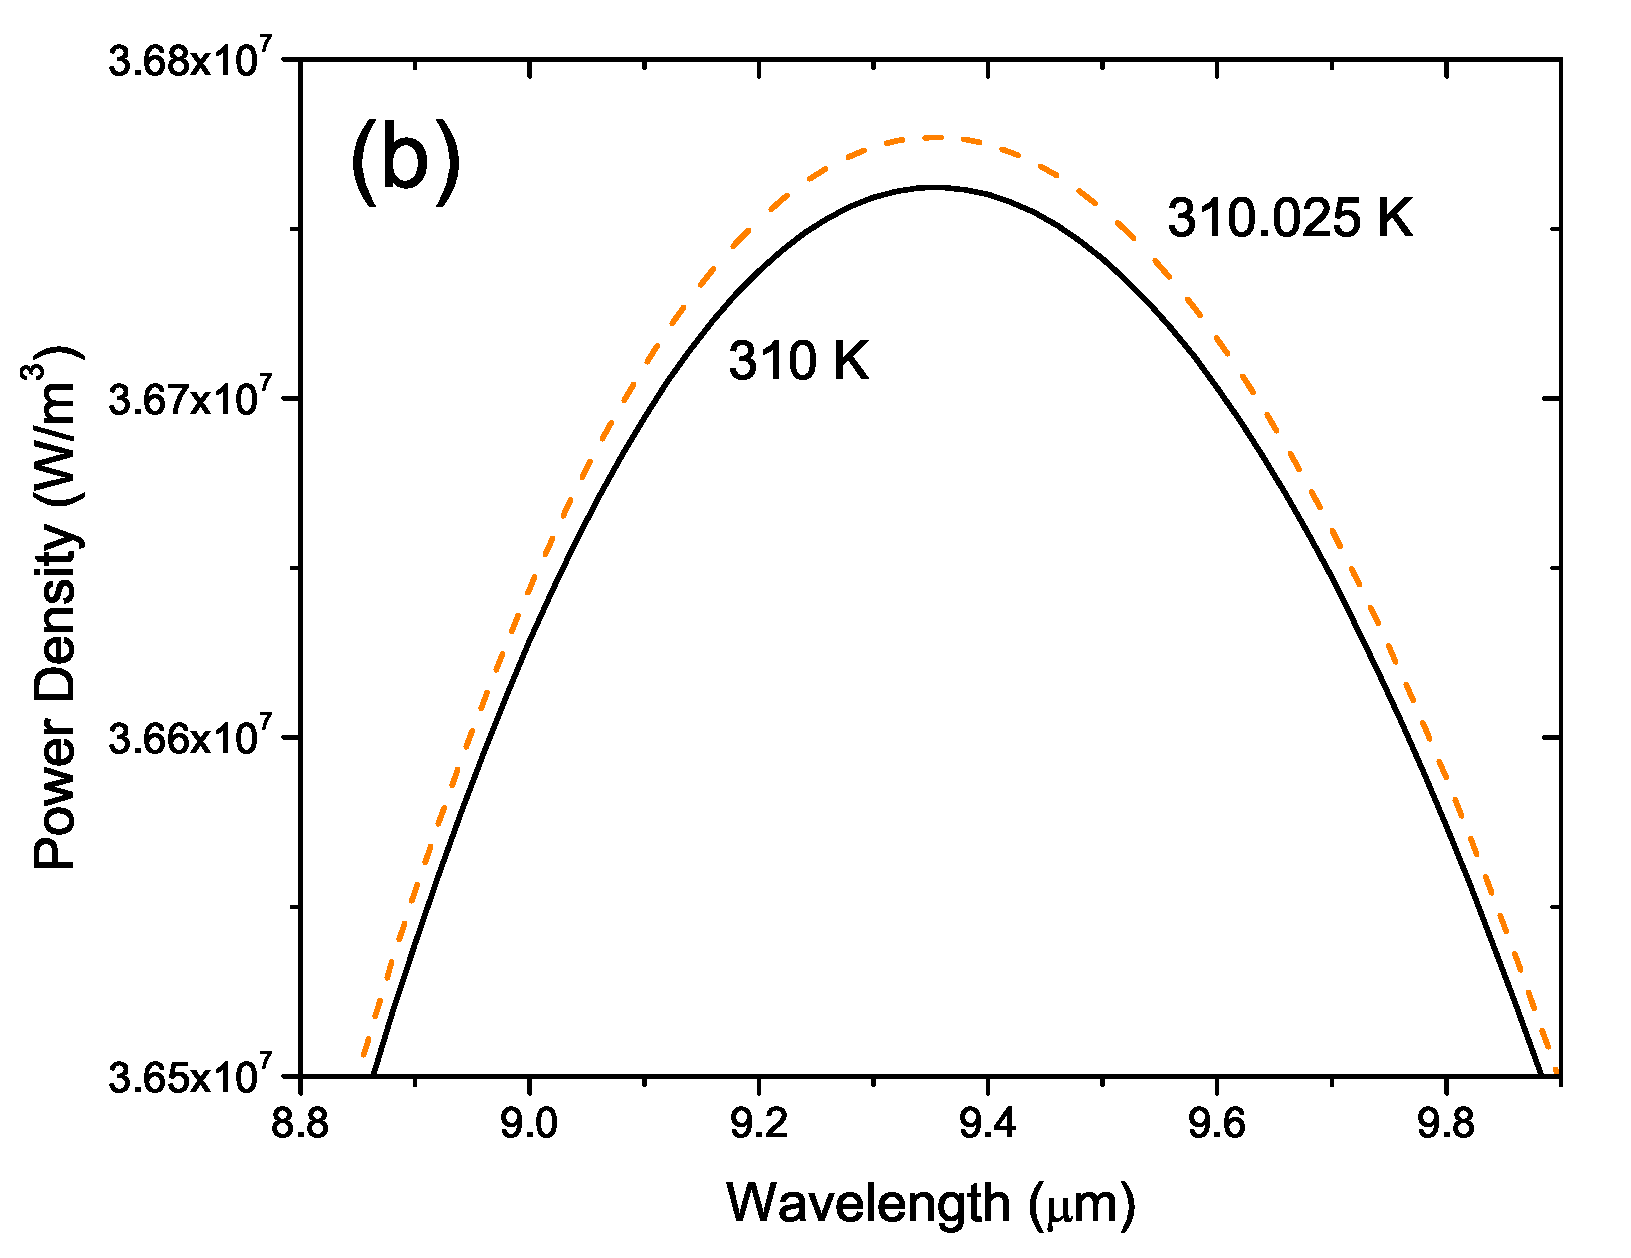
\includegraphics[width=\linewidth]{blackbody-2}
    \end{column}
  \end{columns}
}

\frame{
\frametitle{Black-body Emission}
  \begin{columns}
    \begin{column}{0.2\textwidth}
      \centering
      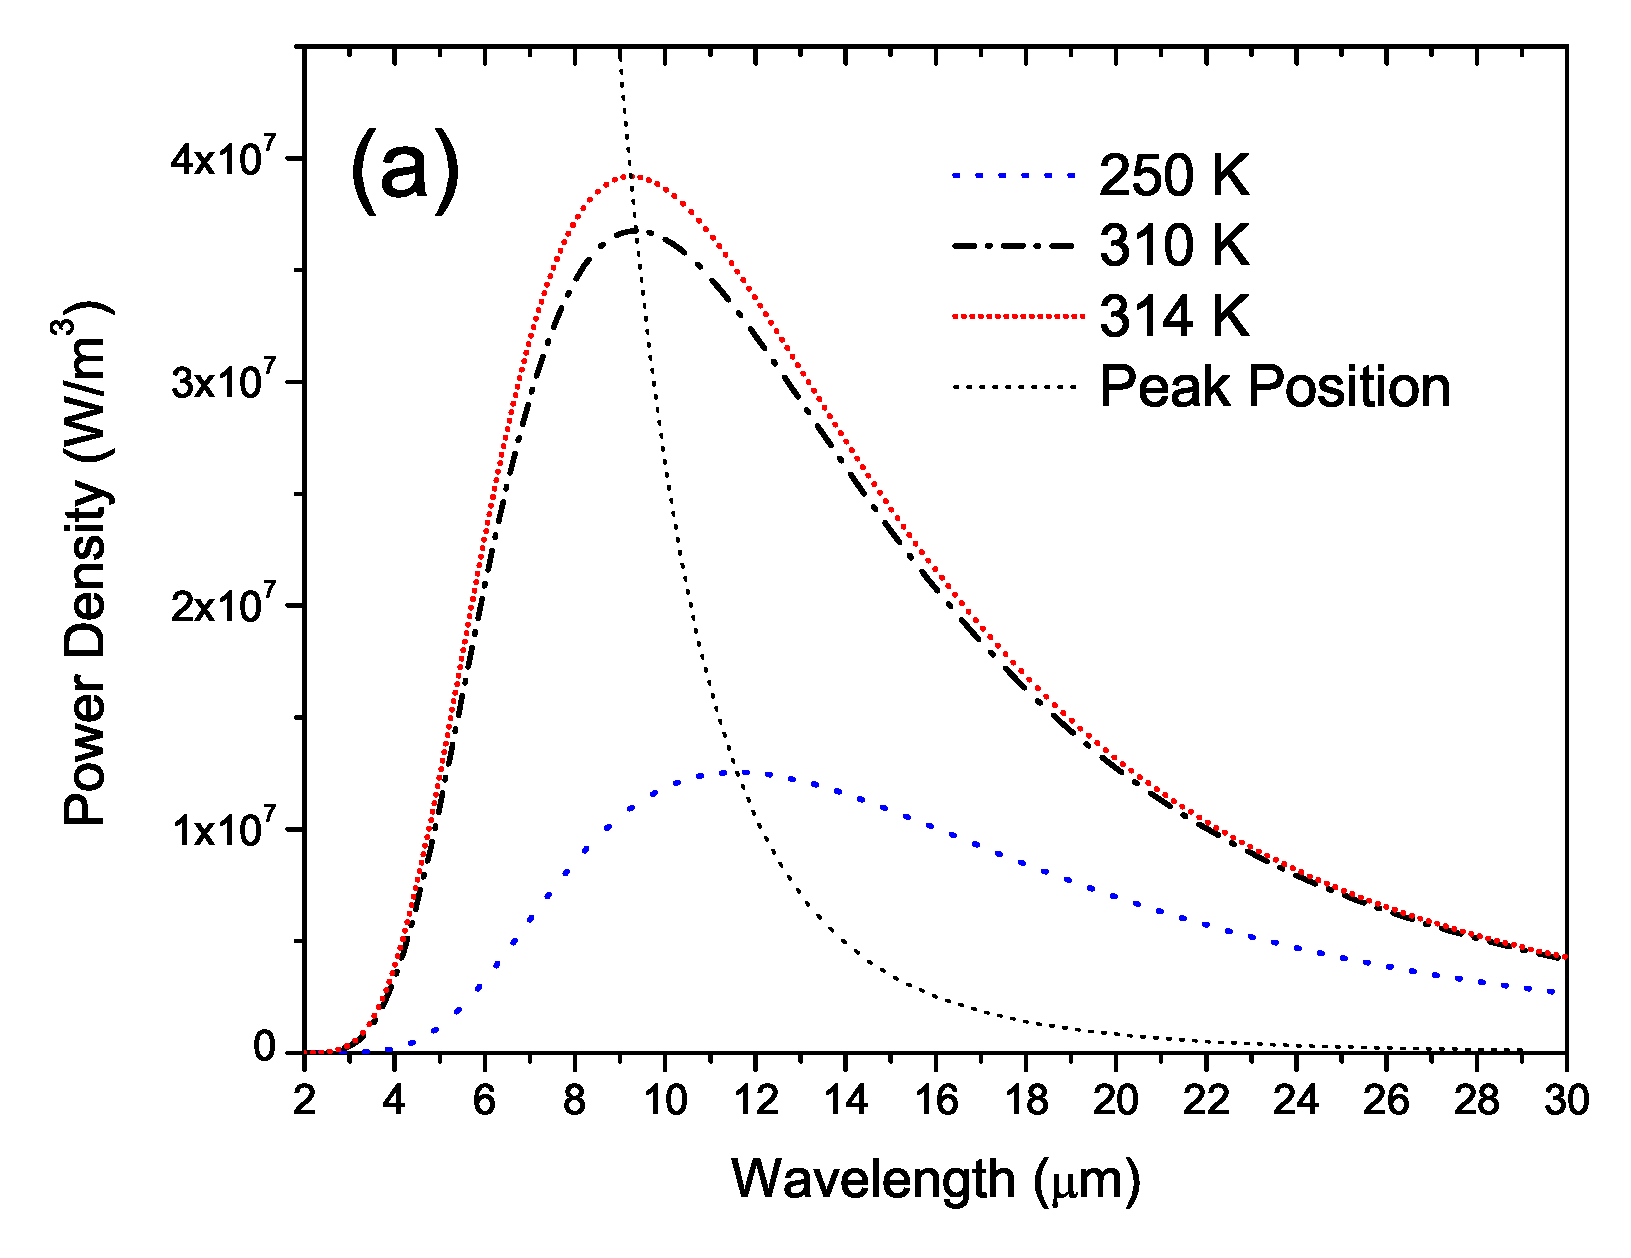
\includegraphics[width=\linewidth]{blackbody-1}
    \end{column}
    \begin{column}{0.8\textwidth}
      \centering
      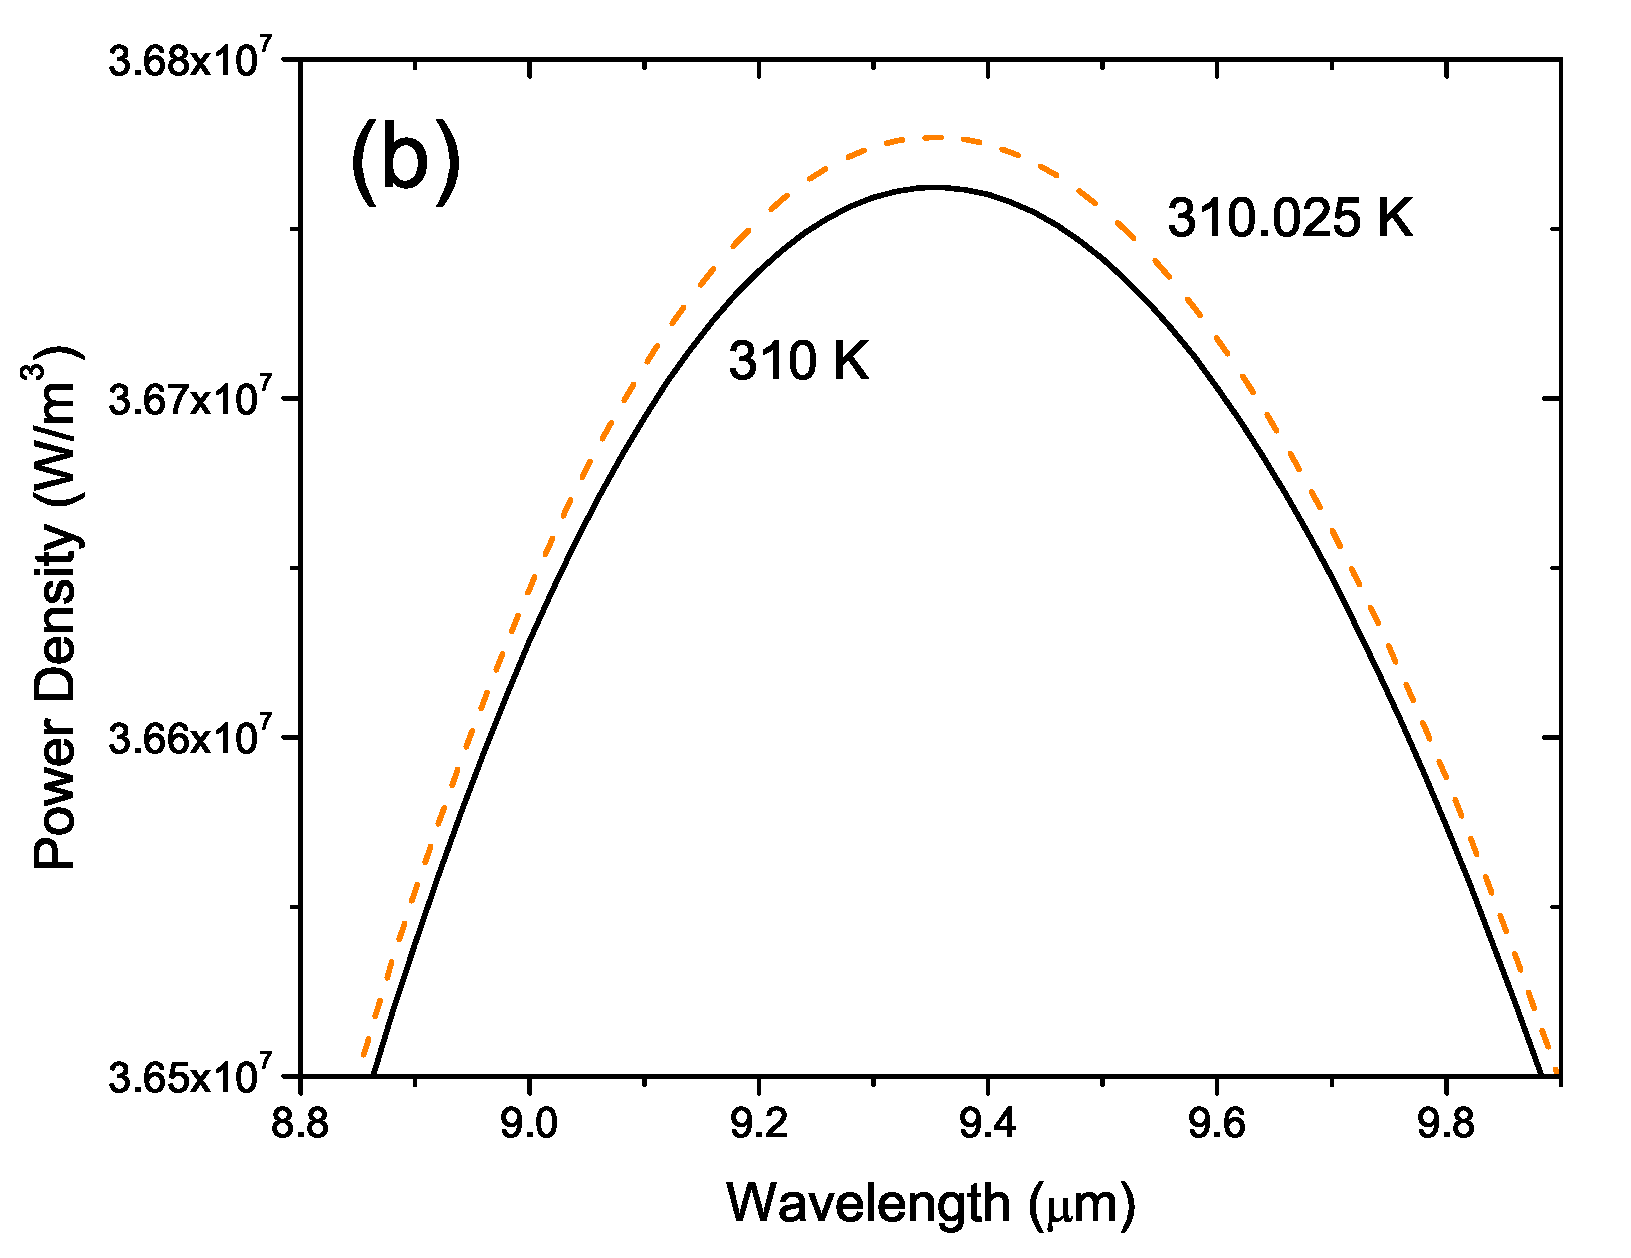
\includegraphics[width=\linewidth]{blackbody-2}
    \end{column}
  \end{columns}
}

\frame{
\frametitle{Broad-band Water Absorption Spectra}
  \centering
  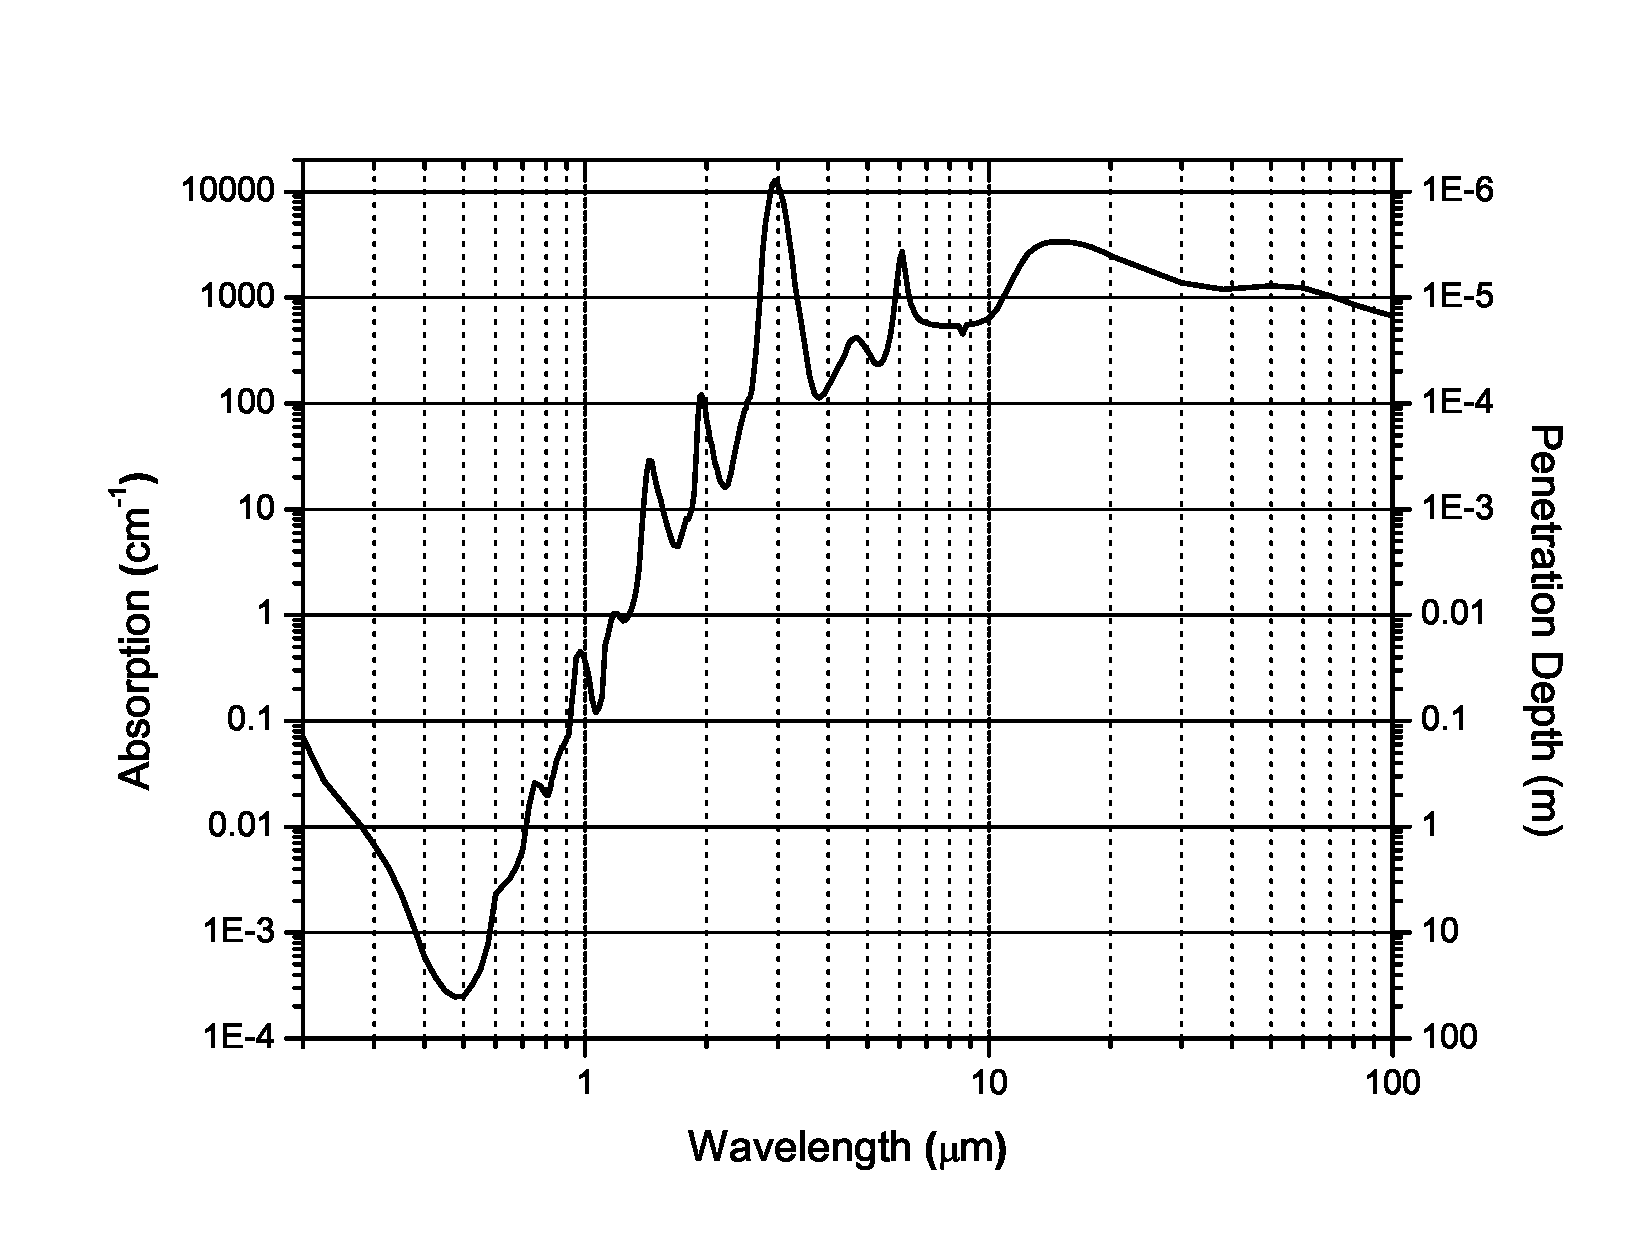
\includegraphics[width=\textwidth]{water-wide-band}
}

%%%%%%%%%%%%%%%%%%%%%%%%%%%%%%%%%%%%%%%%%%%%%%%%%%%%%%%%%%%%%%%
%%%%%  Conclusions
%%%%%%%%%%%%%%%%%%%%%%%%%%%%%%%%%%%%%%%%%%%%%%%%%%%%%%%%%%%%%%%

\frame[plain]{
  \begin{tabularx}{\linewidth}{X}
    \centering
\includegraphics[scale=0.5]{octocat} \\
    \centering
\includegraphics[scale=0.1]{github}
  \end{tabularx}
  \begin{center}
    \vspace*{\fill}
    \Large\texttt{https://github.com/greggroth/temptools}
    \vspace{2cm}
  \end{center}
}

\end{document}